% Options for packages loaded elsewhere
\PassOptionsToPackage{unicode}{hyperref}
\PassOptionsToPackage{hyphens}{url}
%
\documentclass[]{article}
\usepackage{tikz}
\usepackage{amsmath,amssymb}
\usepackage{lmodern}
\usepackage{ifxetex,ifluatex}
\usepackage[margin=0.5cm, landscape]{geometry}
\usepackage{multicol}
\ifnum 0\ifxetex 1\fi\ifluatex 1\fi=0 % if pdftex
  \usepackage[T1]{fontenc}
  \usepackage[utf8]{inputenc}
  \usepackage{textcomp} % provide euro and other symbols
\else % if luatex or xetex
  \usepackage{unicode-math}
  \defaultfontfeatures{Scale=MatchLowercase}
  \defaultfontfeatures[\rmfamily]{Ligatures=TeX,Scale=1}
\fi
% Use upquote if available, for straight quotes in verbatim environments
\IfFileExists{upquote.sty}{\usepackage{upquote}}{}
\IfFileExists{microtype.sty}{% use microtype if available
  \usepackage[]{microtype}
  \UseMicrotypeSet[protrusion]{basicmath} % disable protrusion for tt fonts
}{}
\makeatletter
\@ifundefined{KOMAClassName}{% if non-KOMA class
  \IfFileExists{parskip.sty}{%
    \usepackage{parskip}
  }{% else
    \setlength{\parindent}{0pt}
    \setlength{\parskip}{6pt plus 2pt minus 1pt}}
}{% if KOMA class
  \KOMAoptions{parskip=half}}
\makeatother
\usepackage{xcolor}
\IfFileExists{xurl.sty}{\usepackage{xurl}}{} % add URL line breaks if available
\IfFileExists{bookmark.sty}{\usepackage{bookmark}}{\usepackage{hyperref}}
\hypersetup{
  hidelinks,
  pdfcreator={LaTeX via pandoc}}
\urlstyle{same} % disable monospaced font for URLs
\setlength{\emergencystretch}{3em} % prevent overfull lines
\providecommand{\tightlist}{%
  \setlength{\itemsep}{0pt}\setlength{\parskip}{0pt}}
\setcounter{secnumdepth}{-\maxdimen} % remove section numbering
\ifluatex
  \usepackage{selnolig}  % disable illegal ligatures
\fi

\newcommand{\HRule}[1][\medskipamount]{\par
  \vspace*{\dimexpr-\parskip-\baselineskip+#1}
  \noindent\rule{\linewidth}{0.2mm}\par
  \vspace*{\dimexpr-\parskip-.5\baselineskip+#1}}

\newcommand{\R}{\mathbb R}
\newcommand{\cis}{\operatorname{cis}}
\newcommand{\hl}[1]{\mathversion{bold}\textbf{\textcolor{red!90!green}{#1}}\mathversion{normal}}
\newcommand{\mathlarger}[1]{\displaystyle#1}

\author{}
\date{}

\begin{document}
\pagestyle{empty}
\begin{multicols*}{3}

\subsection{Ordinary differential equations}

A differential equation is an equation where the unknown (or unknowns)
is a function f, and the equation \hl{relates values of f at a point x} with
values of derivatives of the function at \hl{the same point x}. If the
function has one variable only (as is the case in this chapter), one
speaks of ordinary differential equations.

\textbf{Theorem 2.1.6: $F : \mathbb R^2 \rightarrow \mathbb{R}$} is a
differentiable function of two variables. Let $x_0 \in \mathbb{R}$ and
$y_o \in \mathbb R^2$. Then the ODE $y' = F(x,y)$ has an \hl{unique} 
solution $f$ defined on a \emph{largest} open interval $I$
containing $x_0$ such that $f(x_0) = y_0$.

$\exists \ f : I : \mathbb{R}$ s.t.
$\forall x \in I : f'(x) = F(x, y)$ and one cannot find a larger
interval containing $I$ with such a solution.

\textbf{Separation of variables:}

If the ODE can be rewritten as $\frac{dy}{dx}=f(x)g(y)$, then
$$\int\frac{dy}{g(y)}=\int f(x)dx.$$

\hypertarget{linear-differential-equations}{%
\subsection{Linear differential
equations}\label{linear-differential-equations}}

\textbf{Definition 2.2.1:} Let $I \subset \mathbb{R}$ open interval
and $k \geq 1$ an integer.

Homogeneous ODE of order $k$:
$y^{(k)} + a_{k-1}y^{(k-1)} +\dots + a_1y' + a_0 y = 0$ where the
coefficients $a_0, \dots , a_{k-1}$ are complex-valued functions on
$I$.

Inhomogeneous ODE of order $k$:
$y^{(k)} + a_{k-1}y^{(k-1)} +\dots + a_1y' + a_0 y = b$ where
$b : I \rightarrow \mathbb{C}$.


\textbf{Theorem 2.2.3:} Let $I \subset \mathbb{R}$ an open interval
and $k \geq 1$ an integer,

$y^{(k)} + a_{k-1}y^{(k-1)} +\dots + a_1y' + a_0 y = 0$ a linear ODE
over $I$ with continuous coefficients.

\begin{enumerate}
\def\labelenumi{\arabic{enumi}.}
\item
  Set $S$ of k-times differentiable solutions
  $f: I \rightarrow \mathbb{C}$ is a \hl{complex vector space} which is a
  subspace of complex-valued functions on $I$.

  If the functions $a_i$ are real-valued, the set of real-valued
  solutions is also a vector space.
\item
  The dimension of $S$ is $k$, and for any choice of $x_0 \in I$
  and any $(y_0, \dots , y_{k-1}) \in \mathbb C^k$, there exists a
  unique $f \in \mathbb{C}$ such that
  $f(x_0) = y_0, f'(x_0) = y_1, \dots , f^{(k-1)} = y_{k-1}$.
\item
  Let $b$ be a continuous function on $I$. There exists a solution
  $f_0$ to the inhomogeneous equation and the set $S_b$ is the set
  of functions \hl{$f + f_0$} where $f \in S$.
\item
  For any $x_o \in I$ and any
  $(y_0, \dots , y_{k-1}) \in \mathbb C^k$, there exists a unique
  $f \in S_b$ such that
  $f(x_0) = y_0, f'(x_0) = y_1, \dots , f^{(k-1)} = y_{k-1}$.
\end{enumerate}

\hl{If $b \neq 0$, the set $S_b$ is not a vector space!}

\hypertarget{linear-differential-equations-of-order-1}{%
\subsection{Linear differential equations of order
1}\label{linear-differential-equations-of-order-1}}

Let $I \subset \mathbf{R}$ be an open interval. We consider here the
linear differential equation \hl{$y^{\prime}+a y=b$} when $a$ and $b$
are general continuous functions defined on $I$.

Steps to solve:

\begin{enumerate}
\def\labelenumi{\arabic{enumi}.}
\tightlist
\item
  Solve the \hl{homogeneous equation}: $y^{\prime}+a y=0$ and obtain $S$.
\item
  Find solution $f_0$ to the \hl{inhomogeneous equation}.
\item
  $S_b$ will contain $f_0 + f$ where $f \in S$ and if some $f_1$
  is a basis of $S$ then the solutions are given by $f_{0}+z f_{1}$
  where $z \in \mathbb{C}$ are arbitrary.
\end{enumerate}

If the initial value $f(x_0) = y_0$ is given, then one must solve
$f_{0}\left(x_{0}\right)+z f_{1}\left(x_{0}\right)=y_{0}$ and
determine the value of $z$.


\textbf{Proposition 2.3.1:} Any solution of \hl{$y^{\prime}+a y=0$} is of
the form \hl{$f(x)=z \exp (-A(x))$} where $A$ is a primitive of $a$.
The unique solution with $f\left(x_{0}\right)=y_{0}$ is
\hl{$f(x)=y_{0} \exp \left(A\left(x_{0}\right)-A(x)\right)$}.

\subsection{Linear differential equations with constant coefficients}

Now let $k \geq 1$ an integer; $a_0, \dots , a_{k-1}$ constant
coefficients and $b$ a continuous function. We consider the equation
$y^{(k)}+a_{k-1} y^{(k-1)}+\cdots+a_{1} y^{\prime}+a_{0} y=b$.

\textbf{Solution of the homogeneous equation:}

Let
\hl{$P(\lambda)=\lambda^{k}+a_{k-1} \lambda^{k}+\cdots+a_{1} \lambda+a_{0}$}.
Find the \hl{roots} of this polynomial. If the roots are not real but the
coefficients are, express the solution in terms of $\sin$ and $\cos$
using $e^{ix}=\cos x+i \sin x$.

\textbf{Case 1: No multiple roots}

Any solution $f \in S$ of solutions of the homo equation is of the
form \hl{$f(x)=z_{1} e^{\alpha_{1} x}+\cdots+z_{k} e^{\alpha_{k} x}$} for
arbitrary $z_1, \dots , z_k$. To find an unique solution to
$f\left(x_{0}\right)=y_{0}, \ldots, f^{(k-1)}\left(x_{0}\right)=y_{k-1}$
for given $\left(y_{0}, \ldots, y_{k-1}\right)$ just view
$z_1, \dots , z_k$ as unknowns.

To obtain the \hl{real valued solutions} if the coefficients are real:

$f(x)=x_{1} e^{\alpha_{1} x}+\cdots+x_{m} e^{\alpha_{m} x}+ x_{m+1} e^{a_{m+1} x} \cos \left(b_{m+1} x\right)+y_{m+1} e^{a_{m+1} x} \sin \left(b_{m+1} x\right)+\cdots+x_{k} e^{a_{k} x} \cos \left(b_{k} x\right)+y_{k} e^{a_{k} x} \sin \left(b_{k} x\right)$

with $\alpha_1, \dots, \alpha_m$ being the real solutions and
$\alpha_{m+1}, \dots, \alpha_k$ the complex solutions $\alpha_j = a_j + ib_j$.

\textbf{Case 2: Multiple roots}

Assume $\alpha$ is a multiple root of order $j$ of $P$ then the
solutions look as follows:

$f_{\alpha, 0}(x)=e^{\alpha x}, \quad f_{\alpha, 1}(x)=x e^{\alpha x}, \quad \cdots, \quad f_{\alpha, j-1}(x)=x^{j-1} x^{\alpha x}$

That is, multiply the original solution from \emph{Case 1} with
$x^{i-1}$ for $i = 1, \dots , j$.

\textbf{Solution to the inhomogeneous equation:}

\begin{enumerate}
\def\labelenumi{\arabic{enumi}.}
\item
  \textbf{\emph{Ansazt} method} (left side is $b(x)$ and the right
  side is Ansatz)

  $ae^{\alpha x} \rightarrow be^{\alpha x}$

  $a\sin(\beta x)$ or
  $a\cos(\beta x) \rightarrow c\sin(\beta x) + d\cos(\beta )$

  $ae^{\sin(\beta x)}$ or
  $ae^{\cos(\beta x)} \rightarrow e^{\alpha x}[c\sin(\beta x) + d\cos(\beta x)]$

  $P_n(x)e^{\alpha x} \rightarrow R_n(x) e^{\alpha x}$

  $P_ne^{\alpha x}\sin(\beta x)$ or
  $P_ne^{\alpha x}\cos(\beta x) \rightarrow e^{\alpha x}[R_n\sin(\beta x) + S_n\cos(\beta x)]$

  With $P_n(x), R_n(x), Q_n(x), S_n(x)$ being polynomials of degree
  $n$.

  If $b(x)$ is a linear combination of the above functions, then one
  should try the corresponding linear combination of the \emph{Ansatz}
  functions.

  If $\lambda = \alpha + \beta i$ is a root of $P(\lambda)$ of
  multiplicity $m$, then the \emph{Ansatz} function should be
  multiplied by $x^m$ (otherwise the \emph{Ansatz} would solve the
  homo solution again)
\item
  \textbf{Variation of constants}

  Assume $(f_1, \dots , f_k)$ is the basis of the space $S$ of
  solutions of the homogeneous equation. Now we search for a solution of
  the \hl{inhomogeneous equation} of the form
  $f(x)=z_{1}(x) f_{1}(x)+\cdots+z_{k}(x) f_{k}(x)$ and impose the
  following \hl{conditions}:

  $\left\{\begin{array}{l}z_{1}^{\prime}(x) f_{1}(x)+\cdots+z_{k}^{\prime}(x) f_{k}(x)=0 \\z_{1}^{\prime}(x) f_{1}^{\prime}(x)+\cdots+z_{k}^{\prime}(x) f_{k}^{\prime}(x)=0 \\\cdots \\z_{1}^{\prime}(x) f_{1}^{(k-2)}(x)+\cdots+z_{k}^{\prime}(x) f_{k}^{(k-2)}(x)=0\end{array}\right.$
\end{enumerate}

\hypertarget{differential-calculus-in-mathbbrn}{%
\subsection{\texorpdfstring{Differential calculus in
$\mathbb R^n$}{Differential calculus in \textbackslash mathbb\{R\^{}n\}}}\label{differential-calculus-in-mathbbrn}}

\subsubsection{Continuity in $\mathbb R^n$}

The norm $||x||$ satisfies $||x|| > 0$,
$||x|| = 0 \Leftrightarrow x = 0$, $||tx|| = |t|||x||$ for all
$t \in \mathbb{R}$, and $||x+y|| \leq ||x|| + ||y||$ (triangle
inequality).

\textbf{Definition 3.2.1:} Let $(x_k)_{k \in \mathbb{N}}$ where
$x_k \in \mathbb R^n$. $x_k = (x_{k,1}, \dots , x_{k,n})$. Let
$y=(y_1, \dots , y_n)$ . We say that the sequence $(x_k)$ \hl{converges
to $y$} as $y \rightarrow +\infty$ if for all $\epsilon > 0$, there
exists $N \geq 1$ such that for all $n \geq N$ we have
\hl{$||x_k-y|| < \epsilon$}.


\textbf{Lemma 3.2.2:} The sequence $(x_k)$ \hl{converges to $y$} as
$y \rightarrow +\infty \Leftrightarrow$ one of the following holds:

\begin{enumerate}
\def\labelenumi{\arabic{enumi}.}
\tightlist
\item
  For each $1 \leq i \leq n$, the sequence \hl{$(x_{k,i})$} of real
  numbers \hl{converges to $y_i$}.
\item
  The sequence of real numbers \hl{$||x_k - y||$ converges to 0} as
  $y \rightarrow +\infty$.
\end{enumerate}

\textbf{Definition 3.2.3:} Let $X \subset \mathbb R^n$ and
$f:X \rightarrow \mathbb R^m$

\begin{enumerate}
\def\labelenumi{\arabic{enumi}.}
\tightlist
\item
  Let $x_0 \in X$. $f$ is continuous at $x_0$ if for all
  $\epsilon > 0$, there exists $\delta > 0$ such that, if
  $x \in X$ satisfies $||x-x_0|| < \delta$, then
  $||f(x) - f(x_0)|| < \epsilon$.
\item
  $f$ is continuous on $X$ if it is continuous at all $x_0 \in X.$
\end{enumerate}

\textbf{Proposition 3.2.4:} Let $X \subset \mathbb R^n$ and
$f:X \rightarrow \mathbb R^m$. Let $x_0 \in X$. $f$ is \hl{continuous
at $x_0$} $\Leftrightarrow$ for \hl{every sequence} $(x_k)_{k\geq1}$ in
$X$ such that \hl{$x_k \rightarrow x_0$} as $k \rightarrow +\infty$,
the sequence $(f(x_k))_{k\geq 1}$ in $\mathbb R^n$ \hl{converges to
$f(x_0)$}.


\textbf{Definition 3.5.5:} Let $X \subset \mathbb R^n$ and
$f:X \rightarrow \mathbb R^m$. Let $x_0 \in X$ and
$y\in \mathbb R^m$. $f$ has a limit $y$ as $x \rightarrow x_0$
with $x \neq x_0$ if for every $\epsilon > 0$, there exists
$\delta > 0$, such that for all $x \in X$, $x \neq x_0$, such that
$||x-x_0|| < \delta : ||f(x) - y|| < \epsilon$. Then
$\lim _{x \rightarrow x_{0} \atop x \neq x_{0}} f(x)=y$.

\textbf{Proposition 3.2.7:} Let $X \subset \mathbb R^n$ and
$f:X \rightarrow \mathbb R^m$. Let $x_0 \in X$ and
$y\in \mathbb R^m$.

$\displaystyle\lim _{x \rightarrow x_{0} \atop x \neq x_{0}} f(x)=y \Leftrightarrow$
for \hl{every sequence $(x_k)$} in $X$ such that $x_k \rightarrow x$ as
$k \rightarrow +\infty$, and $x_k \neq x_0$, the sequence
$(f(x_k))_{k\geq 1}$ in $\mathbb R^n$ \hl{converges to $y$}.

\textbf{Proposition 2.3.9:} Let
$X \subset \mathbb R^n, Y \subset \mathbb R^m$ and $p \geq 1$ an
integer. Let $f:X\rightarrow Y and g: Y \rightarrow \mathbb{R^p}$ be
\hl{continuous functions}. Then the composition $f \circ g$ is \hl{continuous}.

\hl{Cartesian product, linear maps, multiplication and addition of
continuous functions are continuous.}

If $f:\mathbb R^2\rightarrow\mathbb{R}$ is continuous then so is the
function $g$ defined by $g(x) = f(x,y_0)$ for a fixed $y_0$. The
converse is not true.

\textbf{Definition 3.2.11:} A subset $X \subset \mathbb R^n$ is

\begin{enumerate}
\def\labelenumi{\arabic{enumi}.}
\tightlist
\item
  \hl{Bounded} if the set of $||x||$ for $x \in X$ is bounded in
  $\mathbb{R}$.
\item
  \hl{Closed} if for every sequence $(x_k)$ in $X$ that converges in
  $\mathbb R^n$ to some vector $y\in \mathbb R^n$, we have
  $y\in X$.
\item
  \hl{Compact} if it is bounded and closed.
\end{enumerate}

$\{x\in\mathbb R^n:||x-x_0|| = r, r \geq 0\}$ is closed (same for
$\mathbb R^3$), $\{x\in \mathbb R^n:|f(x)| \leq r, r \geq 0\}$ is
closed. \hl{The union of open sets is open}.


\textbf{Proposition 3.2.13:} Let
$f:\mathbb R^n \rightarrow \mathbb R^m$ be a continuous map. For any
closed set $Y \subset \mathbb R^m$, the set
$f^{-1}(Y)=\{x\in\mathbb R^n : f(x) \in Y\} \subset \mathbb R^n$ is
closed.


\textbf{Theorem 3.2.15:} Let $X \subset \mathbb R^n$, \hl{non empty
compact set} and $f:X \rightarrow Y$ a \hl{continuous} function. Then $f$
is \hl{bounded and achieves its maximum and minimum} $(\exists \ x_+$ and
$x_-$ in $X$ such that $f(x_+) = \sup_x\in X$and
$f(x_-) = \inf_x\in X)$.

\subsubsection{Partial derivatives}

\textbf{Definition 3.3.1:} A subset $X \subset \mathbb R^n$ is \hl{open} 
if, for any $x = (x_1, \dots , x_n) \in X$, $\exists \delta > 0$
such that the set
$\{y = (y_1, \dots , y_n) \in \mathbb R^n : |x_i - xy_i| < \delta \text{ for all }i\}$
is \hl{contained in $X$}.

\textbf{Proposition 3.3.2:} A set $X \subset \mathbb R^n$ is \hl{open} 
$\Leftrightarrow$ the \hl{complement} 
$Y = \{x\in \mathbb R^n:x\notin X\}$ is \hl{closed}.

\textbf{Corollary 3.3.3:} If $f:\mathbb R^n \rightarrow \mathbb R^m$
is continuous and $Y \subset \mathbb R^n$ is open, then $f^{-1}(Y)$
is open in $\mathbb R^n$.

\textbf{Definition 3.3.5:} Let $X \subset \mathbb R^n$ be an \hl{open
set}. Let $f:X \rightarrow \mathbb R^m$. Let $1 \leq i \leq n$.
$f$ has a \hl{partial derivative on $X$ with respect to the $i$-th
variable} if for all $x_0 = (x_{0,1}, \dots , x_{0,n}) \in X$, the
function defined by
$g(t) = f(x_{0,1}, \dots ,x_{0, i-1}, t, x_{0, i+1}, \dots , x_{0,n})$
on the set
$I = \{ t \in R : (x_{0,1}, \dots ,x_{0, i-1}, t, x_{0, i+1}, \dots , x_{0,n}) \in X \}$
\hl{is differentiable at $t = x_{0,i}$}. Its derivative $g'(x_{0,i})$ is
denoted
$\frac{\partial f}{\partial{x_i}}(x_0), \ \partial_{x_i}f(x_0), \ \partial_if(x_0)$.
$g'(t)=(g_1'(t), \dots , g_n'(t))$.

\textbf{Proposition 3.3.7:} $X \subset \mathbb R^n$ \hl{open} and $f, g$
functions from $X$ to $\mathbb R^n$. $1 \leq i \leq n$. If $f$
and $g$ have \hl{partial derivatives with respect to the $i$-th
coordinate on $X$}, then:

\begin{enumerate}
\def\labelenumi{\arabic{enumi}.}
\tightlist
\item
  \hl{$f + g$ also does}, and
  $\partial x_i(f+g) = \partial x_i(f) + \partial x_i(g)$
\item
  \hl{if $m=1$, $fg$ also does} and
  $\partial_{x_i}(fg) = \partial_{ x_i}(f)g + f\partial_{x_i}(g)$.
  Furthermore, if \hl{$g(x) \neq 0$ for all $x \in X$}, then
  \hl{$\frac{f}{g}$ has a partial derivative} with respect to the $i$-th
  coordinate on $X$, with
  $\partial_{x_i}(\frac{f}{g}) = \frac{\partial_{x_i} (f) g - f\partial_{x_i} g}{g^2}$.
\end{enumerate}


\textbf{Definition 3.3.9:} Let $X \subset \mathbb R^n$ be an \hl{open set} 
and $f:X \rightarrow \mathbb R^m$ with partial derivatives on $X$.
$f(x) = (f_1(x), \dots , f_m(x))$. For any $x \in X$, the matrix
$J_f(x) = (\partial_{x_j}f_i(x))_{1 \leq i \leq m \atop 1\leq j \leq n}$is
the \hl{Jacobi matrix} of $f$ at $x$.


\textbf{Definition 3.3.11:} Let $X \subset \mathbb R^n$ be an \hl{open
set} and $f:X \rightarrow \mathbb{R}$. If \hl{all partial derivatives} of
$f$ exists at , then the column vector
$\nabla f(x_0) = \left( \begin{array}{c} \partial_{x_1}f(x_0)\\ \dots\\ \partial_{x_n}f(x_0)\\ \end{array} \right)$
is the \hl{Gradient of $f$ at $x_0$}. The Jacobi matrix for $m = 1$.

\subsubsection{The differential}

\textbf{Definition 3.4.3:} Let $X \subset \mathbb R^n$ be an \hl{open set} 
and $f:X \rightarrow \mathbb R^m$. Let $u$ be a linear map
$\mathbb R^n \rightarrow \mathbb R^m$ and $x_0 \in X$. $f$ is
\hl{differentiable at $x_0$ with differential $u$} if

$$\lim_{x\rightarrow x_0 \atop x\neq 0} \frac{f(x)-f(x_0)-u(x-x_0)}{||x-x_0||}=0$$

where the limit is in $\mathbb R^m$. Denote \hl{$df(x_0) = u$}. If $f$
is differentiable at every $x \in X$ then $f$ is differentiable on
$X$.\hl{The existsence of partial derivatives or directional derivatives
does not guarantee continuity (only the existsence of all partial
derivatives and their continuity does).} 

\textbf{Proposition 3.4.4:} Let $X \subset \mathbb R^n$ be an \hl{open
set} and $f:X \rightarrow \mathbb R^m$ \hl{differentiable on $X$}. Then

\begin{enumerate}
\def\labelenumi{\arabic{enumi}.}
\tightlist
\item
  $f$ is \hl{continuous on $X$}.
\item
  $f$ admits \hl{partial derivatives} with respect to each variable.
\item
  If $m = 1$, let $x_0 \in X$ and
  $u(x_1, \dots , x_n) = a_1x_1, \dots , a_nx_n$ the differential of
  $f$ at $x_0$. Then \hl{$\partial x_if(x_0) = a_i$} for
  $1 \leq i \leq n$.
\end{enumerate}

Let $f,g:\mathbb R^n\rightarrow\mathbb{R}$,
$h(x,y) = (f(x,y), g(x,y))$ and $m(u,v) =uv$, so that
$m\circ h(x,y) = f(x,y)g(x,y)$. Therefore
$\frac{\partial(fg)}{\partial x}=x\partial_xf+u\partial_xg$.

Let $f:I \rightarrow \mathbb R^m$ and
$g:\mathbb R^m \rightarrow \mathbb{R}$, $f$ differentiable on $I$
and $g$ differentiable on $\mathbb R^m$, then $g\circ f$ is
differentiable on $I$ and
\hl{$(g\circ f)'(t)=dg(f(t))f'(t)=\nabla g(f(t))\cdot f'(t)$}.

\textbf{Proposition 3.4.6:} Let $X \subset \mathbb R^n$ be open and
$f:X \rightarrow \mathbb R^m, \, g:X \rightarrow \mathbb R^m$
differentiable on $X$.

\begin{enumerate}
\def\labelenumi{\arabic{enumi}.}
\tightlist
\item
  \hl{$f+g$ is differentiable} with differential $d(f+g) = df + dg$ and
  if $m = 1$ then \hl{$fg$ differentiable}.
\item
  If $m=1$ and $g(x) \neq 0$ for all $x \in X$, then
  \hl{$\frac{f}{g}$ is differentiable}.
\end{enumerate}

\textbf{Proposition 3.4.7:} Let $X \subset \mathbb R^n$ be open and
$f:X \rightarrow \mathbb R^m$. If $f$ has \hl{all partial derivatives} 
on $X$, and if the \hl{partial derivatives are continuous on $X$}, then
$f$ is \hl{differentiable on $X$}. With \hl{$df(x_0) = J_f(x_0)$}.

\textbf{Proposition 3.4.9:} Let $X \subset \mathbb R^n$ and
$Y \subset \mathbb R^m$ be \hl{both open} and
$f : X \rightarrow Y, \, g: Y\rightarrow \mathbb R^p$ \hl{differentiable}.
Then $g \circ f: X \rightarrow \mathbb R^p$ is differentiable on
$X$ and for any $x_0 \in X$, its differential is given by the
composition $d(g\circ f)(x_0)= dg(f(x_0))\circ df(x_0)$, in particular
\hl{$J_{g\circ f}(x_0) = J_g(f(x_0))J_f(x_0)$}.

\textbf{Definition 3.4.11:} Let $X \subset \mathbb R^n$ be open and
$f:X \rightarrow \mathbb R^m$ differentiable. Let $x_0 \in X$ and
$u = df(x_0)$. The graph of the affine linear approximation
\hl{$g(x) = f(x_0) + u(x-x_0)$} from $\mathbb R^n$ to $\mathbb R^m$
is called the \hl{tangent space at $x_0$ to the graph of $f$}.

\textbf{Definition 3.4.13:} Let $X \subset \mathbb R^n$ be open and
$f:X \rightarrow \mathbb R^m$. Let $v \in \mathbb R^n$ be non-zero
vector and $x_0 \in X$. We say that $f$ has a \hl{directional derivative
$w$} $\in \mathbb R^m$ in the \hl{direction $v$}, if $g$ defined on the
set $I = \{t \in \mathbb{R} : x_0 + tv \in X\}$ by
$g(t) = f(x_0 + tv)$ has a derivative at $t=0$, and this is equal to
$w$.

In other words:
$\displaystyle\lim_{t\rightarrow 0 \atop t\neq 0} \frac{f(x_0+tv)-f(x_0)}{t} = \hl{w}$

\hl{Computing}: Let $\varphi(t) = f(x+tv)$, then compute $\varphi'(0)$.
If it doesn't exists, then the directional derivative does not exists.

\textbf{Proposition 3.4.15:} Let $X \subset \mathbb R^n$ be open and
$f:X \rightarrow \mathbb R^m$ \hl{differentiable}. Then for any $x\in X$
and non-zero $v \in \mathbb R^n$, $f$ has a \hl{directional derivative
at $x_0$ in the direction $v$ equal to $df(x_0)(v)$}. Suppose
$m=1$. Let $f:X\rightarrow\mathbb{R}$ be differentiable and $x_0 \in X$.
The \hl{tangent space at $x_0$} to the graph of $f$ is the set of
$(x,y) \in \mathbb R^n\times\mathbb{R}$ such that
\hl{$y=f(x_0)+\nabla f(x_0)\cdot (x-x_0)$}. The vector \hl{$\nabla f(x_0)$
points to the direction of greatest increase}.

The \hl{gradient is perpendicular to the level sets} determined by an
equation of the form $f(x) = c$.

$0=(f\circ \gamma)'(0)=\nabla f(x_0)\cdot \gamma'(0)$.

$D_{v}f(\gamma(t))=df(\gamma(t))v=\nabla f(\gamma(t))\cdot v$.

$\nabla f(x_0)\cdot v=||\nabla f(x_0)||\cos(\theta)$ where $\theta$ is
the angle between the gradient and the direction $v$.

\subsubsection{Higher derivatives}

\textbf{Definition 3.5.1:} Let $X \subset \mathbb R^n$ be open and
$f:X \rightarrow \mathbb R^m$. $f$ is of class \hl{$C^1$} if $f$ is
\hl{differentiable on $X$} and \hl{all its partial derivatives are continuous}.
The set of functions of class $C^1$ from $X$ to $\mathbb R^m$ is
denoted $C^1(X;\mathbb R^m)$. Let $k \geq 2$, then $f$ is of
class $C^k$ if it is differentiable and each partial derivative
$\partial x_if:X\rightarrow \mathbb R^m$ is of class $C^{k-1}$. If
$f \in C^k(C;\mathbb R^m)$ for all $k \geq 1$, then
$f \in C^{\infty}$.

\textbf{Proposition 3.5.4:} Let $k \geq 2$, $X \subset \mathbb R^n$
be open and $f:X \rightarrow \mathbb R^m \in C^k$. Then the partial
derivatives of order $k$ are \hl{independent of the order in which the
partial derivatives were taken}: For any $x$ and $y$,
$\partial{x,y}f=\partial{y, x}f$. Same for more variables.

\textbf{Definition 3.5.8:} Let $X \subset \mathbb R^n$ be open and
$f:X \rightarrow \mathbb{R} \in C^2$. For $x\in X$, the \hl{Hessian
matrix} of $f$ at $x$ is the \hl{symmetric square matrix} 
$\text{Hess}_f(x) = (\partial_{x_i, x_j}f)_{1\leq i \atop j \leq n} = H_f(x)$.
$$
\operatorname{Hess}_f(x)=
  \begin{pmatrix}
    \frac{\partial^2 f}{\partial x_1^2}&\hdots&\frac{\partial^2 f}{\partial x_1 x_n}\\
    \vdots&\ddots&\vdots\\
    \frac{\partial^2 f}{\partial x_n x_1}&\hdots&\frac{\partial^2 f}{\partial x_n^2}
  \end{pmatrix}
$$

\subsubsection{Change of variable}

We have an open set $U \subset \mathbb R^n$ with
$(y_1, \dots , y_n)$ the new variables and a change of variable
$g:U \rightarrow X$ which expresses the variables
$(x_1, \dots , x_n)$ \hl{in terms of the new variables}. For a given
function $f : X \rightarrow \mathbb{R}$, the composite
$h= f\circ g:U \rightarrow \mathbb{R}$ is $f$ expressed in terms of
the new variables $y$.

$$\partial_{y_1}h = \frac{\partial f}{\partial x_1}\frac{\partial g_1}{\partial y_1} + \dots +  \frac{\partial f}{\partial x_n}\frac{\partial g_n}{\partial y_1}$$

Some common notation: $\partial_{y_1}h = \partial_{y_1}f$ since they
are the same function with different coordinate systems. $g_i$ is
usually also replaced with $x_i$, s.t.
$\partial_{y_1}f = \frac{\partial f}{\partial x_1}\frac{\partial g_1}{\partial y_1} + \dots + \frac{\partial f}{\partial x_n}\frac{\partial g_n}{\partial y_1} = \frac{\partial f}{\partial x_1}\frac{\partial x_1}{\partial y_1} + \dots + \frac{\partial f}{\partial x_n}\frac{\partial x_n}{\partial y_1}$

\subsubsection{Taylor polynomials}

\textbf{Definition 3.7.1:} Let $k \geq 1$ be an integer and
$f:X\rightarrow \mathbb{R}$ a function of class $C^k$ on $X$ and
some fix $x_0\in X$. The $k$-th Taylor polynomial of $f$ at
$x_0$ is the polynomial in $n$ variables of degree $\leq k$ given
by

$\displaystyle T_kf(y;x_0)=f(x_0)+\sum^{n}_{i=1}\frac{\partial f}{\partial x_i}y_i+\dots + \sum_{m_1 + \dots  + m_n= k}\frac{1}{m_1!\cdot\cdot\cdot m_n!}\frac{\partial^kf}{\partial x_ {1}^{m_1}\cdot\cdot\cdot \partial x_ {n}^{m_n}}(x_0)y_{1}^{m_1}\cdot\cdot\cdot y_n^{m_n}$, such that for $y=x-x_0 : f(x)=T_kf(x-x_0;x_0) + \text{(remainder)} $.

$\displaystyle\frac{1}{2} \sum_{i=1}^{n} \partial_{x_{i}^{2}}^{2} f\left(x_{0}\right) y_{i}^{2}+\sum_{1 \leqslant i<j \leqslant n} \partial_{x_{i} x_{j}}^{2} f\left(x_{0}\right) y_{i} y_{j}=\frac{1}{2} y^{t} \operatorname{Hess}_{f}\left(x_{0}\right) y$
hence \hl{$$T_2f(y;x_0)=f(x_0)+\nabla f(x_0)\cdot y + \frac{1}{2} y^{t} \operatorname{Hess}_{f}\left(x_{0}\right)\cdot y,$$} 
for $y \in \mathbb {R}$.

\textbf{Proposition 3.7.3:} Let $k \geq 1$ be an integer,
$X \subset \mathbb R^n$ be open and $f:X\rightarrow \mathbb{R}$ a
function of class $C^k$. For $x_0 \in X$, if we define
$E_kf(x;x_0)$ by $f(x) = T_kf(x-x_0;x)+E_kf(x;x_0)$ then
$\displaystyle\lim_{x \rightarrow x_0 \atop x\neq x_0}\frac{E_kf(x;x_0)}{||x-x_0||^k} =0$.

\subsubsection{Critical points}

\textbf{Proposition 3.8.1:} Let $X \subset \mathbb R^n$ be open and
$f:X\rightarrow \mathbb{R}$ differentiable. If $x_0 \in X$ s.t.

$f(y) \leq f(x_0)$ for all $y$ close enough to $x_0$ (local
maximum at $x_0)$

or $f(y) \geq f(x_0)$ for all $y$ close enough to $x_0$ (local
minimum at $x_0)$

then \hl{$df(x_0) = 0$} , $\nabla f(x_0)=0$ or
$\partial_{x_i}f(x_0) = 0$ equivalently for $1 \leq i \leq n$.

\textbf{Definition: 3.8.2:} Let $X \subset \mathbb R^n$ be open and
$f:X\rightarrow \mathbb{R}$ differentiable. A point $x_0 \in X$ s.t.
\hl{$\nabla f(x_0) = 0$} is called a \hl{critical point} of $f$.

When $f$ is defined on a compact set $\bar{X} = X \cup B$ with $X$
an open set and $B$ the boundary, then the maxima and minima should
also be explicitly \hl{computed at the boundary}.

\textbf{Definition 3.8.6:} Let $X \subset \mathbb R^n$ be open and
$f:X\rightarrow \mathbb{R}$ of class $C^2$. A critical point
$x_0 \in X$ of $f$ is \hl{non-degenerate} if the \hl{Hessian matrix has
non-zero determinant}.

\textbf{Corollary 3.8.7:} Let $X \subset \mathbb R^n$ be open and
$f:X\rightarrow \mathbb{R}$ of class $C^2$, $x_0 \in X$ a
non-degenerate critical point of $f$. Let $p$ and $q$ be the
positive and negative eigenvalues of $\text{Hess}_f(x_0)$.

\begin{enumerate}
\def\labelenumi{\arabic{enumi}.}
\tightlist
\item
  If $p=n$, $f$ has a local \hl{minimum} at $x_0$.
\item
  If $q=n$, $f$ has a local \hl{maximum} at $x_0$.
\item
  Otherwise, $f$ has a \hl{saddle point} at $x_0$.
\end{enumerate}

$p = n \Leftrightarrow H_f(x_0)$ is positive definite.

$A=(a_{i,j})_{1\leq i \atop j\leq n}$ is \hl{positive definite
$\Leftrightarrow \det(A_k) > 0$} for $1 \leq k \leq n$.
A is \hl{negative definite $\Leftrightarrow (-1)^k\det(A_k)>0$} for $1 \leq k \leq n$.

\subsection{Integration in $\mathbb R^n$}

\hypertarget{line-integrals}{%
\subsubsection{Line integrals}\label{line-integrals}}

\textbf{Definition 4.1.1:}

\begin{enumerate}
\def\labelenumi{\arabic{enumi}.}
\tightlist
\item
  Let $I = [a, b]$ a closed and bounded interval in $\mathbb{R}$.
  Let $f(t)=(f_1(t), \dots , f_n(t))$ continuous from $I$ to
  $\mathbb R^n$. Then we define
  $\int_a^bf(t)dt=(\int_a^b(f_1(t), \dots , f_n(t)) \in \mathbb R^n$.
\item
  A \hl{parameterised curve} in $\mathbb R^n$ is a continuous map
  $\gamma:[a,b] \rightarrow \mathbb R^n$ that is piecewise $C^1$.
\item
  Let $\gamma:[a,b] \rightarrow \mathbb R^n$ be a parameterised
  curve. Let $X \subset \mathbb R^n$ be a subset containing the image
  of $\gamma$, and let $f:X \rightarrow \mathbb R^n$ continuous.
  \hl{$$\int_a^bf(\gamma(t))\cdot \gamma'(t)dt \in \mathbb{R}$$} is called
  the line integral of $f$ along $\gamma$. It is denoted
  $\int_{\gamma}f(s)ds$ or $\int_{\gamma}f(s)d\vec{s}$.
\end{enumerate}

For $X\subset \mathbb R^n$, $f:X\rightarrow \mathbb R^n$ is usually called 
a \hl{vector field}.

\textbf{Definition 4.1.4:} Let $\gamma:[a,b] \rightarrow \mathbb R^n$
be a parameterised curve. An oriented reparametrisation of $\gamma$ is
a parameterised curve $\sigma:[c,d] \rightarrow \mathbb R^n$ such
that $\sigma =\gamma \circ \varphi$ where
$\varphi : [c,d] \rightarrow [a,b]$ is a continuous map,
differentiable on $]a,b[$, that is strictly increasing and satisfies
$\varphi(a) = c$ and $\varphi(b)=d$.

\textbf{Proposition 4.1.5:} Let $\gamma$ be a \hl{parameterised curve} in
$\mathbb R^n$ and $\sigma$ an \hl{oriented reparametrisation} of
$\gamma$. Let $X$ be a set containing the image of $\gamma$, or
equivalently the image of $\sigma$, and
$f: X\rightarrow \mathbb R^n$ continuous. Then we have
$\int_{\gamma}f(s)\cdot d\vec{s} = \int_{\sigma}f(s)\cdot d\vec{s}$.

\textbf{Definition 4.1.8:} Let $X \subset \mathbb R^n$ and
$f:X \rightarrow \mathbb R^n$ a \hl{continuous vector field}. If for any
$x_1, x_2$ in $X$, the \hl{line integral} 
$\int_\gamma f(c)\cdot d\vec s$ is \hl{independent of the choice of a
parameterised curve} $\gamma$ in $X$ from $x_1$ to $x_2$, then we
say that the vector field is \hl{conservative}.

Equivalently, $f$ is conservative
$\Leftrightarrow$ \hl{$\int_\gamma f(s) \cdot d \vec s= 0$} for any \hl{closed} 
parameterised curve in $X$. Where a curve is closed if
$\gamma(a) = \gamma(b)$.

\textbf{Theorem 4.1.10:} Let $X$ be an open set and $f$ a
\hl{conservative} vector field. Then there exists a $C^1$ function $g$ on
$X$ such that \hl{$f = \nabla g$}. If any two points of $X$ are
conjoined by a parameterised curve, then g is unique up to addition of a
constant: if $\nabla g_1=f$, then $g-g_1$ is constant on $X$.

Any two points $x$ and $y$ on $X$ can be \hl{joined by a parameterised
curve} $\Leftrightarrow \exists \gamma:[a,b] \rightarrow X$ such that
$\gamma(a) = x$ and $\gamma(b) = y$. Then $X$ is \hl{path connected}.
This is also true whenever $X$ is convex. If $f$ is conservative,
then a function g such that $\nabla g= f$ is called a \hl{potential for
$f$}.

$$\int_a^bf(\gamma(t))\cdot \gamma'(t)dt \in \mathbb{R} = g(\gamma(b)) - g(\gamma(a))$$

A set $X$ is \hl{convex} if for any $x, y \in X$, the line segment
joining $x$ to $y$ is contained in $X$.

\textbf{Proposition 4.1.13:} Let $X \subset \mathbb R^n$ be an open
set and $f:X \rightarrow \mathbb R^n$ of class $C^1$.

$f(x)=(f_1(x), \dots , f_n(x))$. If $f$ is \hl{conservative}, then we
have
\hl{$\frac{\partial f_i}{\partial x_j}=\frac{\partial f_j}{\partial x_i}$}
for any integers with $1 \leq i \neq j \leq n$.

\textbf{Definition 4.1.15:} A subset $X \subset \mathbb R^n$ is \hl{star-shaped}
if there exists $x_0 \in X$ such that, for all $x \in X$, the
\hl{line segment joining $x_0$ to $x$ is contained in $X$}. We then say
that $X$ is star-shaped around $x_0$.


\textbf{Theorem 4.1.17:} Let $X$ be a \hl{star-shaped} open subset of
$\mathbb R^n$ and $f$ a $C^1$ vector field such that
\hl{$\frac{\partial f_i}{\partial x_j}=\frac{\partial f_j}{\partial x_i}$}
on $X$ for all $i\neq j$ between $1$ and $n$. Then the vector
field $f$ is \hl{conservative}.

The requirement that $X$ is star-shaped is not necessary. $X$ should have
no “hole” in the middle around which a circle can go without it being
possible to contract it within $X$.

\textbf{Definition 4.1.20:} Let $X\subset \mathbb R^3$ be an open set
and $f:X \rightarrow \mathbb R^3$ a $C^1$ \hl{vector field}. Then the
\hl{curl} of $f$, denoted $\text{curl}(f)$, is the continuous vector
field on $X$ defined by
$$\displaystyle\text{curl}(f)=\left(
\begin{array}{c}
\partial_{y}f_3 - \partial_zf_2\\
\partial_zf_1 - \partial_x f_3\\
\partial_xf_2-\partial_yf_1\\
\end{array}
\right)$$
where $f(x, y, z)=(f_1(x,y,z), f_2(x,y,z), f_3(x,y,z))$.

$$\operatorname{curl}(f)=
\begin{vmatrix}
  e_1 & e_2 & e_3\\
  \partial_x & \partial_y & \partial_z\\
  f_1 & f_2 & f_3\\
\end{vmatrix}$$
with the rule that $\partial_x \cdot f_i = f_i \cdot \partial_x = \partial_xf_i$.

\hl{$\operatorname{curl}(\nabla f)=0$}.

\subsubsection{The Riemann integral in $\mathbb R^n$}

The goal is to define the integral $\int_Xf(x_1, \dots , x_n)dx$ for a
closed and bounded set $X$ and continuous function $f$, so that it
has analogue properties to the Riemann integral for $n=1$.

For a bounded and closed subset $X \subset \mathbb R^n$ and any
continuous function $f:X \rightarrow \mathbb{R}$, one can define the
integral of $f$ over $X$ denoted $\int_Xf(x)dx$, which is a real
number.

The integral satisfies the following properties:

\begin{enumerate}
  \def\labelenumi{\arabic{enumi}.}
  \tightlist
\item
  \textbf{Compatibility:}
  If \textbf{$n=1$} and $X=[a,b]$ with
  $a\leq b$, then $$\int_{[a,b]}f(x)dx=\int_a^bf(x)dx$$.
\item
  \textbf{Linearity:}
  If $f$ and $g$ are continuous on $X$ and
  $a,b \in \mathbb{R}$, then
  $$\int_X(af_1(x)+bf_2(x))dx = a\int_Xf_1(x)dx+b\int_Xf_2(x)dx$$.
\item
  \textbf{Positivity:} If $f\leq g$, then
  $$\int_Xf(x)dx\leq\int_Xg(x)dx$$ and especially, if $f \geq 0$, then
  $$\int_Xf(x)dx \geq 0.$$ Moreover, if $Y \subset X$ is compact and
  $f\geq 0$, then $$\int_Yf(x)dx\leq\int_Xf(x)dx.$$
\item
  \textbf{Upper bound and triangle inequality:} In particular, since
  $-|f|\leq f \leq |f|$, we have
  $$\left| \int_Xf(x)dx \right| \leq \int_X|f(x)|dx,$$ and since
  $|f+g| \leq |f| + |g|$, we have
  $$\left| \int_X(f(x)+g(x))dx \right| \leq \int_X|f(x)|dx + \int_X|g(x)|dx.$$
\item
  \textbf{Volume:} If $f=1$, then the integral of $f$ is the
  volume in $\mathbb R^n$ of the set $X$, and if $f\geq 0$
  in general, the integral of $f$ is the volume of the set
  $\{(x,y) \in X \times \mathbb{R} : 0 \leq y \leq f(x)\} \subset \mathbb R^{n+1}$.
  In particular, if $X$ is a bounded rectangle, say
  $X = [a_1,b_1] \times \dots \times [a_n, b_n] \subset \mathbb R^n$
  and if $f=1$, then $$\int_Xdx=(b_n-a_n) \cdot\cdot\cdot(b_1-a_1).$$
\item
  \textbf{Multiple integral or Fubini's Theorem:} If $n_1$ and $n_2$
  are integers $\geq 1$ such that $n=n_1+n_2$, then for
  $x_1 \in\mathbb R^n$, let
  $$Y_{x_1} = \{x_2\in\mathbb R^{n_2}:(x_1, x_2)\in X\} \subset \mathbb R^{n_2}.$$
  Let $X_1$ be the set of $x_1 \in \mathbb R^n$ such that
  $Y_{x_1}$ is not empty. Then $X_1$ is compact in
  $\mathbb R^{n_1}$ and $Y_{x_1}$ is compact in
  $\mathbb R^{n_2}$ for all $x_1\in X_1$. If the function
  $$g(x_1)=\int_{Y_{x_1}}f(x_1,x_2)dx_2$$ on $X_1$ is continuous, then
  $$\int_Xf(x_1,x_2)dx=\int_{X_1}g(x_1)dx_1$$
  $$=\int_{X_1}\left(\int_{Y_{x_1}}f(x_1,x_2)dx_2\right)dx_1.$$
  Similarly, exchanging the role of $x_1$ and $x_2$, we have
  $$\int_{X} f\left(x_{1}, x_{2}\right) d x=\int_{X_{2}}\left(\int_{Z_{x_{2}}}
  f\left(x_{1}, x_{2}\right) d x_{1}\right) d x_{2}$$
  where
  $Z_{x_{2}}=\left\{x_{1}:\left(x_{1}, x_{2}\right) \in X\right\}$, if
  the integral over $x_1$ is a continuous function.
\end{enumerate}

If the variables are $x_1, \dots , x_n$ we also write
$\int_Xf(x_1, \dots\ , x_n)dx_1, \dots\ , dx_n$

\textbf{Definition 4.2.3:}

\begin{enumerate}
\def\labelenumi{\arabic{enumi}.}
\tightlist
\item
  Let $1\leq m \leq n$ be an integer. A parameterised $m$-set in
  $\mathbb R^n$ is a \hl{continuous map} 
  $f:[a_1,b_1]\times \dots \times[a_m,b_m] \rightarrow \mathbb R^n$
  which is $C^1$ on $]a_1, b_1[ \times \dots \times ]a_m,b_m[$.
\item
  A subset $B\subset \mathbb R^n$ is \hl{negligible} if there exists an
  integer $k \geq 0$ and parameterised $m_i$-sets
  $f_i:X_1 \rightarrow \mathbb R^n$, with $1\leq i \leq k$ and
  $m_i < n$, such that $X\subset f_1(X_1) \cup \dots\ \cup f_k(X_k)$ .
\end{enumerate}

The \hl{image} of a parameterised $m$-set $f$ might be of \hl{dimension
smaller than $m$} (e.g. if $f$ is constant, in which case the image
is a single point, which is an object of dimension 0)

\textbf{Proposition 4.2.5:} Let $X\subset \mathbb R^n$ be compact.
Assume that $X$ is \hl{negligible}. Then for any continuous function on
$X$, we have \hl{$\int_Xf(x)dx=0$}.

\subsubsection{Improper integrals}

Let $I \subset \mathbb{R}$ be a \hl{bounded interval}, $J=[a, +\infty[$
for some $a\in \mathbb{R}$ and $f$ a \hl{continuous function} on
$X=J \times I$. We say that it is \hl{Riemann-intrgrable} on $X$ if the
limit

$$\lim _{x \rightarrow+\infty} \int_{[a, x] \times I} f(x, y) d x d y=\lim _{x \rightarrow+\infty} \int_{a}^{x}\left(\int_{I} f(x, y) d y\right) d x$$
$$=\lim _{x \rightarrow+\infty} \int_{I}\left(\int_{a}^{x} f(x, y) d x\right) d y$$

exists. Denote this limit by $$\int_{J\times I}f(x,y)dxdy.$$ Similarly
let $f$ be continuous on $\mathbb R^2$. Assume that $f\geq 0$.
$f$ is Riemann-integrable on $\mathbb R^2$, if the limit
$$\lim_{R\rightarrow+\infty}\int_{[-R,R]^2}f(x,y)dxdy$$
exists, which is called the integral of $f$ over $\mathbb R^2$ and
denoted $$\int_{R^2}f(x,y)dxdy.$$ This integral is also the limit of
$$\int_{D_R}f(x,y)dxdy$$ where $D_R$ is the disc of radius $R$
centred at $0$.

The easiest way to prove that a certain \hl{improper integral exists}: If
$|f| \leq g$ (resp $0\leq f \leq g)$, and
$$\int_{J \times I} g(x, y) d x d y$$ or
$$\int_{\mathbf{R}^{2}} g(x, y) d x d y$$ exists, then so
does $$\int_{J\times I}f(x,y)dxdy \text{ or } \int_{R^2}f(x,y)dxdy.$$

\subsubsection{The change of variable formula}

Let $\bar X \subset \mathbb R^n$ and $\bar Y \subset \mathbb R^n$
be \hl{compact subsets}, $\varphi:\bar X \rightarrow \bar Y$ a \hl{continuous
map}. We assume that we can write $\bar X=X\cup B, \bar Y=Y\cup C$
where

\begin{enumerate}
\def\labelenumi{\arabic{enumi}.}
\tightlist
\item
  $X$ and $Y$ are \hl{open} 
\item
  $B$ and $C$ are \hl{negligible} 
\item
  the restriction of $\varphi$ to the open set $X$ is a $C^1$
  \hl{bijective map from $X$ to $Y$}.
\end{enumerate}

In this situation, the Jacobian matrix $J_{\varphi}(x)$ is \hl{invertible
at all $x\in X$}.

\textbf{Theorem 4.4.2:} In the situation described above, for any
continuous function $f$ on $\bar Y$, we have
\hl{$\int_{\bar X}f( \varphi)|\det(J_{\varphi}(x))|dx=\int_{\bar Y}f(y)dy$}.

\textbf{Cartesian to polar coordinates:}
\hl{$x=r\cos(\theta), y=r\sin(\theta)$}, then calculate all partial derivatives with respect
to the new variables:

$\partial_rx=\cos\theta, \partial_ry=\sin\theta, \partial_\theta x=-r\sin\theta,
\partial_\theta y=r\cos\theta$. Then \hl{$J_{(r, \theta)}=r, dxdy \rightarrow rdrd\theta$}.

\subsubsection{Geometric applications of integrals}

\begin{enumerate}
\def\labelenumi{\arabic{enumi}.}
\item
  \textbf{Centre of mass:}

  Let $X$ be a compact subset of $\mathbb R^n$, such that the
  volume of $X$ is positive. The centre of mass of $X$ is the point
  $\bar x \in \mathbb R^n$ such that
  $\bar x =(\bar x_1, \dots\ , \bar x_n)$ with
  $$\bar x_i = \frac{1}{\text{vol}(X)}\int_Xx_idx.$$ Intuitively,
  $\bar x_i$ is the average over $X$ of the $i$-th coordinate, and
  $\bar x$ is the point where $X$ is perfectly balanced.

  Note that $\bar x$ is not necessarily in $X$.
\item
  \textbf{Surface area:}

  Consider the continuous function
  $f:[a,b] \times [c,d] \rightarrow \mathbb{R}$ which is $C^1$ on
  $]a,b[\times]c,d[$. Let
  $$\Gamma = \{(x,y,z) \in \mathbb R^3 : (x,y) \in [a,b]\times [c,d], z=f(x,y)\}$$
  $\subset\mathbb R^3$
  be the graph of $f$. This is a surface and should have an area,
  which is given by
  $$\int_a^b\int_c^d\sqrt{1+(\partial_xf(x,y))^2+(\partial_yf(x,y))^2}dxdy.$$
\item
  \textbf{Length of a curve:}

  $$f:[a,b] \rightarrow \mathbb{R}:\int_a^b\sqrt{1+f'(x)^2}dx.$$
\end{enumerate}

\subsubsection{The Green formula}

The Green formula concerns the case of \hl{relating an integral over a
subset} $X$ of $\mathbb R^2$ with a \hl{line integral over its boundary}.

\textbf{Definition 4.6.1:} A \hl{simple closed parameterised curve} 
$\gamma:[a,b] \rightarrow \mathbb R^2$ is a closed parameterised
curve such that \hl{$\gamma(t)\neq \gamma(s)$} unless $t=s$ or
$\{s,t\} = \{a,b\}$, and such that $\gamma'(t)\neq 0$ for
$a < t < b$. If $\gamma$ is only piecewise $C^1$ inside $]a,b[$,
this condition only applies to where $\gamma'(t)$ exists.

\textbf{Theorem 4.6.3:} Let $X\subset \mathbb R^2$ \hl{compact with a
boundary $\partial X$} that is the union of finitely many simple closed
parameterised curves $\gamma_1, \dots\ , \gamma_k$. Assume that
$\gamma_i:[a_i,b_i] \rightarrow \mathbb R^2$ has the property that
$X$ lies always \hl{to the left} of the tangent vector
$\gamma_i'(t)$ based at $\gamma_i(t)$. Let $f=f(f_1, f_2)$ be a
vector field of class $C^1$ defined on some open set containing $X$.
Then we have
$$\int_X\left(\frac{\partial f_2}{\partial x}-\frac{\partial f_1}{\partial y}\right)dxdy = \sum_{i=1}^k\int_{\gamma_i}f\cdot d\vec s.$$

\textbf{Corollary 4.6.5:} Let $X\subset \mathbb R^2$ compact with a
boundary $\partial X$ that is the union of finitely many simple closed
parameterised curves $\gamma_1, \dots\ , \gamma_k$. Assume that
$\gamma_i:[a_i,b_i] \rightarrow \mathbb R^2$ has the property that
$X$ lies always \hl{to the left} of the tangent vector
$\gamma_i'(t)$ based at $\gamma_i(t)$. Then we have
$$\operatorname{Vol}(X)=\sum_{i=1}^{k} \int_{\gamma_{i}} x \cdot d \vec{s}=\sum_{i=1}^{k} \int_{a_{i}}^{b_{i}} \gamma_{i, 1}(t) \gamma_{i, 2}^{\prime}(t) dt.$$

\subsubsection{The Gauss-Ostrogradski formula}

This formula is the analogue of the Green formula in $\mathbb R^3$.

\textbf{Definition 4.7.1:} A \hl{parameterised surface} 
$\Sigma : [a,b]\times [c,d] \rightarrow \mathbb R^3$ is a $2$-set
in $\mathbb R^3$ such that the \hl{rank of the Jacobian matrix is $2$}
at all $(s,t)\in]a,b[\times]c,d[$.

\textbf{Definition 4.7.3:} Let $x$ and $y$ be two \hl{linearly
independent} vectors in $\mathbb R^3$. The vector product, or \hl{cross
product} $z=x\times y$ is the unique vector in $\mathbb R^3$ such
that $(x,y,z)$ is a basis of $\mathbb R^3$ with
$\det(x,y,z) > 0$, and $||z||=||x|| \, ||y|| \sin(\theta)$, where
$\theta$ is the angle between $x$ and $y$.

$x \times y=\left(\begin{array}{l}x_{2} y_{3}-x_{3} y_{2} \\x_{3} y_{1}-x_{1} y_{3} \\x_{1} y_{2}-x_{2} y_{1}\end{array}\right)=\operatorname{det}\left|\begin{array}{lll}e_{1} & e_{2} & e_{3} \\x_{1} & x_{2} & x_{3} \\y_{1} & y_{2} & y_{3}\end{array}\right|$

$e_1 \times e_2 = e_3, \ e_2\times e_3 = e_1, \ e_3 \times e_1 = e_2$
and $y \times x = -x \times y$

\textbf{Theorem 4.7.6:} Let $X\subset \mathbb R^3$ \hl{compact with a
boundary $\partial X$} that is a parameterised surface
$\Sigma:[a,b]\times [c,d] \rightarrow\mathbb R^3.$ Assume that
$\Sigma$ is injective in $]a,b[\times ]c,d[$, and that $\Sigma$
has the property that the normal vector $\vec n$ points away from
$\Sigma$ at all points. Let $\vec u = \frac{\vec n}{||\vec n||}$ be
the unit exterior normal vector. Let $f=(f_1, f_2, f_3)$ be a vector
field of class $C^1$ defined on dome open set containing $X$. Then
we have
$$\int_X\operatorname{div}(f)dxdydz = \int_\Sigma(f\cdot \vec u)d\sigma.$$

For a vector field $f=(f_1, f_2, f_3)$ on $X\subset \mathbb R^3$,
we denote the \hl{divergence of the field} 
$\operatorname{div}(f)=\partial_xf+\partial_yf+\partial_zf$.

For a parameterised surface
$\Sigma:[a,b]\times [c,d] \rightarrow\mathbb R^3$ with exterior
normal vector field
$\vec n = (n_1, n_2, n_3) = \partial_s\Sigma\times\partial_t\Sigma$
and a function $g$ defined on the image of $\Sigma$, we define the
\hl{surface integral}
$$\int_\Sigma g \ d\sigma = \int_a^b\int_c^dg(\Sigma(s,t))\sigma(s,t)dsdt$$
where
$\sigma(s,t)=||\partial_s\Sigma\times\partial_t\Sigma||=||\vec n(s,t)||$.

Like the integral for a parameterised curve, the surface integral is
\hl{independent of the chosen parmeterisation of the surface}.

For a $C^1$ vector field $f=(f_1,f_2,f_3)$ on $\mathbb R^3$, we
define $$\int_\Sigma (f\cdot \vec n)d\sigma=\int_\Sigma g \ d\sigma,$$ where
$$g(\Sigma(s,t))=f(\Sigma(s,t))\cdot \vec u(s,t) = \sum_{i=1}^3u_i(s,t)f_i(\Sigma(s,t)).$$
This is called the \hl{flux of the vector field} $f$ through the surface
$\Sigma$.

In the flux, $\vec u(s,t)\sigma(s,t)=\vec n(s,t)$.

\subsection{Examples and other}

\subsubsection{Basic rules that you will forget :)}

\textbf{Complex Numbers}

$ e^{i\varphi} = \cos(\varphi) + i\sin(\varphi) $, $e^{i\varphi} = \cis(\varphi)$, $\vert e^{i\varphi}\vert = 1$

\resizebox{\columnwidth}{!}{\begin{tabular}{|l|l|l|}
  \hline
  $z$ & $ z = x + iy  \left\{
  \begin{array}{l}
  \text{x: Real}\\ \text{y: Imaginary}
  \end{array}
  \right. $  & $z = r \cdot e^{i\varphi} = r \cdot \cis(\varphi)  $\\ 
  \hline
  $\overline{z}$ & $\overline{z} = x - iy$ & $z = r \cdot e^{-i\varphi}$\\ 
  \hline
  $\vert z \vert$ & $\vert z \vert = \sqrt{z \cdot \overline{z}} = \sqrt{x^{2} + y^{2}}$ & $\vert z \vert = r =\sqrt{z \cdot \overline{z}}$\\ 
  \hline
  $z_1 + z_2$ & $x_1+x_2 + i(y_1+y_2)$ & \\
  \hline
  $z_1 - z_2$ & $x_1-x_2 + i(y_1-y_2)$ & \\
  \hline
  $z_1 \cdot z_2$ & $(x_1x_2 - y_1y_2) + i(x_1y_2 + x_2y_1)$ & $r_1 \cdot r_2 \cdot 
  e^{i(\varphi_1+\varphi_2)}$\\
  \hline
  $\frac{z_1}{z_2}, z_2 \neq 0$ & $\frac{z_1 \cdot \overline{z_2}}{\vert z_2 \vert ^{2}} = \frac{(x_1x_2+y_1y_2)+i(x_2y_1-x_1y_2)}{x_2^{2}+y_2^{2}} $ & $\frac{r_1}{r_2} \cdot e^{i(\varphi_1 - \varphi_2)}$\\
  \hline
  $\frac{1}{z}, z \neq 0$ & $\frac{\overline{z}}{\vert z \vert ^{2}} = \frac{(x)+iy}{x^{2}+y^{2}} $ & $\frac{1}{r} \cdot e^{-i\varphi}$\\
  \hline
\end{tabular}}

\resizebox{\columnwidth}{!}{\begin{tabular}{|l|l|}
  \hline
  $z^{n}$ & $r^{n} \cdot (\cos(n\cdot \varphi)+ i \sin(n \cdot \varphi)) = r^{n} \cdot e^{in\varphi}$\rule{0pt}{2.6ex}\\
  \hline
  $\sqrt[n]{z}$ & $\sqrt[n]{r}\cdot(\cos(\frac{\varphi + 2\pi k}{n})) + i\sin(\frac{\varphi + 2 \pi k }{n}), \ k = 0, 1, ..., n-1 $ \rule{0pt}{2.6ex}\\
  \hline
\end{tabular}}

\scalebox{0.85}{\begin{tabular}{|l|l|l|l|}
  \hline $i^{0}$ & $i^{1}$ & $i^{2}$ & $i^{3}$\\
  \hline $1$ & $i$ & $-1$ & $-i$\\
  \hline
\end{tabular}}

\textbf{Abs:}

  $\vert ab \vert = \vert a \vert \vert b\vert $  
  $\vert \frac{a}{b} \vert = \frac{\vert a \vert}{ \vert b\vert} $ 
  $\vert a + b \vert \le \vert a \vert + \vert b \vert$ \\

\textbf{Power rules:}

$x = \sqrt[n]{a} \Leftrightarrow\ (x^{n} = a \ \text{and } x \ \ge 0)$ \;
$\sqrt[n]{-a} = - \sqrt[n]{a}, \ a \ge 0$ \;
$a^{-n} = \frac{1}{a^{n}} = (\frac{1}{a})^{n}$ \;
$a^{\frac{1}{n}} = \sqrt[n]{a}$ \;
$\sqrt{ab} = \sqrt{a}\sqrt{b}$ \;
$a^{\frac{m}{n}} = \sqrt[n]{a^{m}}$ \;
$ \sqrt{\frac{a}{b}} = \frac{\sqrt{a}}{\sqrt{b}} $ \;
$ a^{x} = e^{x \cdot \ln a}$ \;
$\sqrt[n]{a^{-m}} = \frac{1}{\sqrt[n]{a^{m}}}$ \;
$a^{m}a^{n} = a^{m+n} $ \;
$\sqrt[n]{a^{m}} = \sqrt[kn]{a^{km}}$ \;
$\frac{a^{m}}{a^{n}} = a^{m-n}$ \;
$ \sqrt[n]{\sqrt[k]{a}} = \sqrt[nk]{a}$ \;
$(a^{m})^{n} = a^{mn}$ \;
$\sqrt[n]{a}\sqrt[n]{b} = \sqrt[n]{ab}$  \;
$a^{n}b^{n} = (ab)^{n}$ \;
$\frac{\sqrt[n]{a}}{\sqrt[n]{b}} = \sqrt[n]{\frac{a}{b}}$  \;
$\frac{a^{n}}{b^{n}} = (\frac{a}{b})^{n}$  \;

\textbf{Differentiation:}

\begin{itemize}
  \item \textbf{Sum} $(f(x)+g(x))' = f'(x) + g'(x)$
  \item \textbf{Factor} $(c\cdot f(x))' = c\cdot f'(x)$
  \item \textbf{Product} $(f(x)\cdot g(x))' = f'(x)g(x) + f(x)g'(x)$
  \item \textbf{Quotient} $\left(\frac{f(x)}{g(x)}\right)' = \frac{f'(x)g(x) - f(x)g'(x)}{g^2(x)} \ (g\neq 0)$
  \item \textbf{Chain Rule} $(f(g(x)))' = (f\circ g)' = f'(g(x))g'(x)$
\end{itemize}

\textbf{Integration:}

\begin{itemize}
  \item $\int_a^b (f(x) +/- g(x)) xd = \int_a^b f(x) +/- \int_a^b g(x)$
  \item $\int_a^b c\cdot f(x)dx = c\cdot \int_a^b f(x)dx$
  \item $\int_a^b f'(x)\cdot g(x)dx = \left[f(x)g(x)\right]_a^b - \int_a^b f(x)g'(x)$
  \item $\int_{\phi(a)}^{\phi(b)} f(x)dx = \int_a^b f(\phi(t))\phi '(t) dt$
  \item \textbf{$a+c, b+c \in I$} $\int_a^b f(t+c)dt = \int_{a+c}^{b+c} f(x)dx$
  \item \textbf{$ca,cb\in I$: } $\int_a^b f(ct)dt = \frac{1}{c}\int f(x)dx$
  \item $\int\frac{f'(t)}{f(t)}dt = \log(|f(x)|)$, bzw. $\int_a^b\frac{f'(t)}{f(t)}dt = \log(f(|b|)) - \log(f(|a|))$
  \item \textbf{Partial fraction:}\\
  $\frac{2x^6-4x^5+5x^4-3x^3+x^2+3x}{(x-1)^3(x^2+1)^2} = \frac{A}{x-1}+\frac{B}{(x-1)^2}+\frac{C}{(x-1)^3}+\frac{Dx+E}{x^2+1}+\frac{Fx+G}{(x^2+1)^2}$
  \item \textbf{Substitution:}\\
  $\int_a^b f(x) dx = \int_{g^{-1}(a)}^{g^{-1}(b)} f(g(u)) g'(u) du$\\

  $\int_{\Omega} f(x,y) dx dy=$\\$\int_{\widetilde{\Omega}} f(g(u, v), \; h(u, v)) \, 
		    \left\lvert\det \, \underbrace{\begin{pmatrix}
			    \frac{\partial g}{\partial u} & \frac{\partial g}{\partial v}\\
			    \frac{\partial h}{\partial u} & \frac{\partial h}{\partial v}
		    \end{pmatrix}}_{d\Phi = \nabla\Phi} \right\rvert
	    ~ du dv$
\end{itemize}

\textbf{Coordinate transformations:}

Polar Coordinates in $\R^2$
\begin{alignat*}{4}
  x &= r \cos \varphi \quad &&0 \leq r < \infty \quad &&&dxdy = r \cdot drd\varphi\\
  y &= r \sin \varphi \quad &&0 \leq \varphi < 2\pi &&&
\end{alignat*}
Elliptic Coordinates $\R^2$
\begin{alignat*}{4}
  x &= r \cdot  a \cos \varphi\quad &&0 \leq r < \infty\quad &&&dxdy = a \cdot b \cdot  r \cdot drd\varphi\\
  y &= r \cdot b \sin \varphi\quad &&0 \leq \varphi < 2\pi &&&
\end{alignat*}
Cylinder Coordinates $\R^3$ \begin{alignat*}{4}
  x &= r \cdot  a \cos \varphi\quad &&0 \leq r < \infty &&&dxdydz = r \cdot drd\varphi dz\\
  y &= r \cdot b \sin \varphi\quad &&0 \leq \varphi < 2\pi\\
  z &= z\quad &&\-\infty \leq z < \infty\quad
\end{alignat*}
Sphere Coordinates $\R^3$ \begin{alignat*}{4}
  x &= r \cdot \sin \theta \cos \varphi \quad &&0 \leq r < \infty \quad &&&dxdydz = r^2 \sin \theta \cdot drd\theta d\varphi\\
  y &= r \cdot \sin \theta \sin \varphi \quad && 0 \leq \theta < \pi &&&\\
  z &= r \cos \theta \quad &&0 \leq \varphi < 2\pi &&&
\end{alignat*}

\textbf{Limits:}

\begin{itemize}
  \item $\lim_{x\to 0} \arctan(x) = 0$, $\lim_{x\to\infty} \arctan(x) = \frac{\pi}{2}$
  \item $\lim_{x\to 0} \tan(x) = 0$, $\lim_{x\to\infty} \tan(x) = \infty$, $\lim_{x\to\frac{\pi}{2}} \tan(x) = \infty$
  \item $\lim_{x\to\infty}{\cos(x)=[-1, 1]}$, $\lim_{x\to\infty}{\sin(x)=[-1, 1]}$
  \item $\lim_{n \to \infty}{(1+\frac{x}{n})^{n}} = e^{x}$  $\lim_{n \to \infty}{(1+\frac{1}{n})^{n}} = \lim_{n\to\infty}{(1+n)^{\frac{1}{n}}} = e$ 
  \item $\lim_{x\to 0}{\frac{a^{x}-1}{x}} = \ln(a)$  $\lim_{x\to 0}\frac{\log_a(1+x)}{x} = \frac{1}{\ln(a)}$  $\lim_{x \to 0}{\frac{1-\cos(x)}{x}} = 0$ 
  \item $ \lim_{x\to 0}{\frac{1-\cos(x)}{x^{2}}} = \frac{1}{2} $  $ \lim_{x\to 0}{\frac{\tan(x)}{x}} = 1$  $ \lim_{x\to 0}{\frac{\sin(x)}{x}} = 1 = \frac{x}{\sin(x)}$ 
  \item $\lim_{x\to\infty}{\frac{n!}{n^{n}}} = 0$  $\lim_{x\to 0}{\frac{e^{n} -1}{n}} = 1$  $\lim_{x\to\infty}{\sqrt[n]{n!}} = \infty$  $\lim_{x\to\infty} {\sqrt[n]{n}} = 1$
\end{itemize}

\textbf{Obvious cases:}

$\frac{1}{0} = \infty$ \ $\frac{1}{\infty} = 0$ \ $\infty + \infty = \infty$ \
$0 + \infty = \infty$ \ $0^{\infty} = 0$ \ $\infty^{\infty} = \infty$

\textbf{Sums:}

\begin{itemize}
  \item $\sum_{k=0}^{\infty} aq^{k} = a + aq + aq^{2} +... = \frac{a}{1-q}$ (Geometric Series)
  \item $\sum_{k=0}^{\infty} (k+1)q^{k} = 1 + 2q + 3q^{2} +... = \frac{1}{(1-q)^{2}}, \ \vert q \vert < 1$ 
  \item $\sum_{k=0}^{\infty} \frac{(-1)^{k}}{2k+1} = 1 - \frac{1}{3} + \frac{1}{5} - \frac{1}{7} + ... = \frac{\pi}{4}$
  \item $\sum_{k=1}^{\infty} \frac{1}{k^{2}} = 1 + \frac{1}{2^{2}} + \frac{1}{3^{2}} + \frac{1}{4^{2}} + ... = \frac{\pi^{2}}{6}$
  \item $\zeta(a) = \sum_{k=0}^{\infty} \frac{1}{k^{a}} \text{ist konvergent} \iff a>1$
  \item $\sum_{k=0}^{\infty} \frac{1}{k!} = 1+\frac{1}{1!} + \frac{1}{2!} + \frac{1}{3!} + ... = e$
  \item $\sum_{k=0}^{\infty} \frac{(-1)^{k}}{k!} = 1 - \frac{1}{1!} + \frac{1}{2!} - \frac{1}{3!} + ... = \frac{1}{e}$
  \item $\frac{1}{1 \pm x} = 1 \mp x + x^2 \mp x^3 + x^4 \mp ...$
  \item $\frac{1}{(1 \pm x)^2} = 1 \mp 2x + 3x^2 \mp 4x^3 + 5x^4 \mp ...$
  \item $\sqrt{1 \pm x} = 1 \pm \frac{x}{2} - \frac{\scriptstyle{1\cdot 1}}{\scriptstyle{2 \cdot 4}}x^2 \pm \frac{\scriptstyle{1\cdot 1 \cdot 3}}{\scriptstyle{2 \cdot 4 \cdot 6}}x^3 - \frac{\scriptstyle{1 \cdot 1 \cdot 3 \cdot 5}}{\scriptstyle{2 \cdot 4 \cdot 6 \cdot 8}}x^4 \pm \scriptstyle\cdots$
  \item $\exp(x) = \sum_{n=0}^{\infty} \frac{x^{n}}{n!} = 1 + x + \frac{x^{2}}{2!} + \frac{x^{3}}{3!} + ....$
  \item $\sin(x) =  \sum_{n=0}^{\infty} (-1)^{n}\frac{x^{2n+1}}{(2n +1)!} = x - \frac{x^{3}}{3!} + \frac{x^{5}}{5!} - \frac{x^{7}}{7!} + ...$ 
  \item $\cos(x) =  \sum_{n=0}^{\infty} (-1)^{n}\frac{x^{2n}}{(2n)!} = 1 - \frac{x^{2}}{2!} + \frac{x^{4}}{4!} - \frac{x^{6}}{6!} + ...$ 
  \item $\sinh(x) = \sum_{n=0}^{\infty} \frac{x^{2n+1}}{(2n+1)!} = x + \frac{x^3}{3!} + \frac{x^5}{5!} + ...$
  \item $\cosh(x) = \sum_{n=0}^{\infty} \frac{x^{2n}}{(2n)!} = 1 + \frac{x^2}{2!} + \frac{x^4}{4!} + ...$
  \item $\tan(x) = 1 + \frac{\phi^3}{3} + \frac{2\phi^5}{15} + ...$
  \item $\tanh(z) = 1 \pmb{-} \frac{z^3}{3} \pmb{+} \frac{2z^5}{15} \pmb{-} ...$
  \item $\ln(1+z) = \sum_{k=1}^{\infty} \frac{(-1)^{k+1}}{k}z^k = z - \frac{z^2}{2} + \frac{z^3}{3} + ...$
  \item $(1+z)^\alpha = \sum_{k=0}^{\infty}  \binom{\alpha}{k} z^k = 1 + \alpha z + \frac{\alpha(\alpha - 1)}{2!} z ^ 2 + ...$
\end{itemize}

\textbf{Random:}

\begin{itemize}
  \item Circle formula: $(x - x_0)^2 + (y - y_0)^2 = r^2$
  \item Ellipse formula: $\frac{(x-x_0)^2}{a^2} + \frac{(y-y_0)^2}{b^2} = 1$
  \item Quadratic formula: $x_{1, 2} = \frac{-b \pm \sqrt{b^2 - 4ac}}{2a}$
  \item Determinant: $\begin{vmatrix}
    a & b\\
    c & d
  \end{vmatrix} = ad-bc$
  \item Matrix is invertible iff. the Determinant $\neq 0$.
  \item Scalar Product: $x \cdot y = \sum_{i=1}^n x_i y_i$
  \item Crosss Product: $a \times b = (a_2b_3-a_3b_2, ~~~ a_3b_1-a_1b_3, ~~~ a_1b_2-a_2b_1)^\top$
\end{itemize}

Let $L$ be a \hl{continuous linear function}, then if $L$ is continuous at some
point $x_0$, it is continuous at every point.
$\displaystyle \lim_{x\rightarrow 0}||L(a+x)-L(a)|| = \lim_{x \rightarrow 0} ||L(a) + L(x)-L(a)|| = \lim_{x\rightarrow0} ||L(x)|| = \lim_{x \rightarrow0} ||L(x_o+x) -L(x_0)||=0$.

\textbf{Finding limits:}

\begin{enumerate}
\def\labelenumi{\arabic{enumi}.}
\tightlist
\item
  Different paths
\item
  If $f$ is continuous then
  $\displaystyle\lim_{x\rightarrow a}f(g(x)) = f(\lim_{x\rightarrow a}g(x))$
\item
  Squeeze theorem
\item
  Taylor expansion
\item
  Polar coordinates:\\
  $\displaystyle x = r\cos(\phi), y=r\sin(\phi), \lim_{(x,y)\rightarrow (0,0)}\frac{x^2+y^2}{4x^2+y^6}=\lim_{r\rightarrow0}\frac{r^2}{4r^2\cos^4(\phi)+r^6\sin^6(\phi)}$
\end{enumerate}

\subsection{Sin and Cos}
\begin{center}
\resizebox{\columnwidth}{!}{
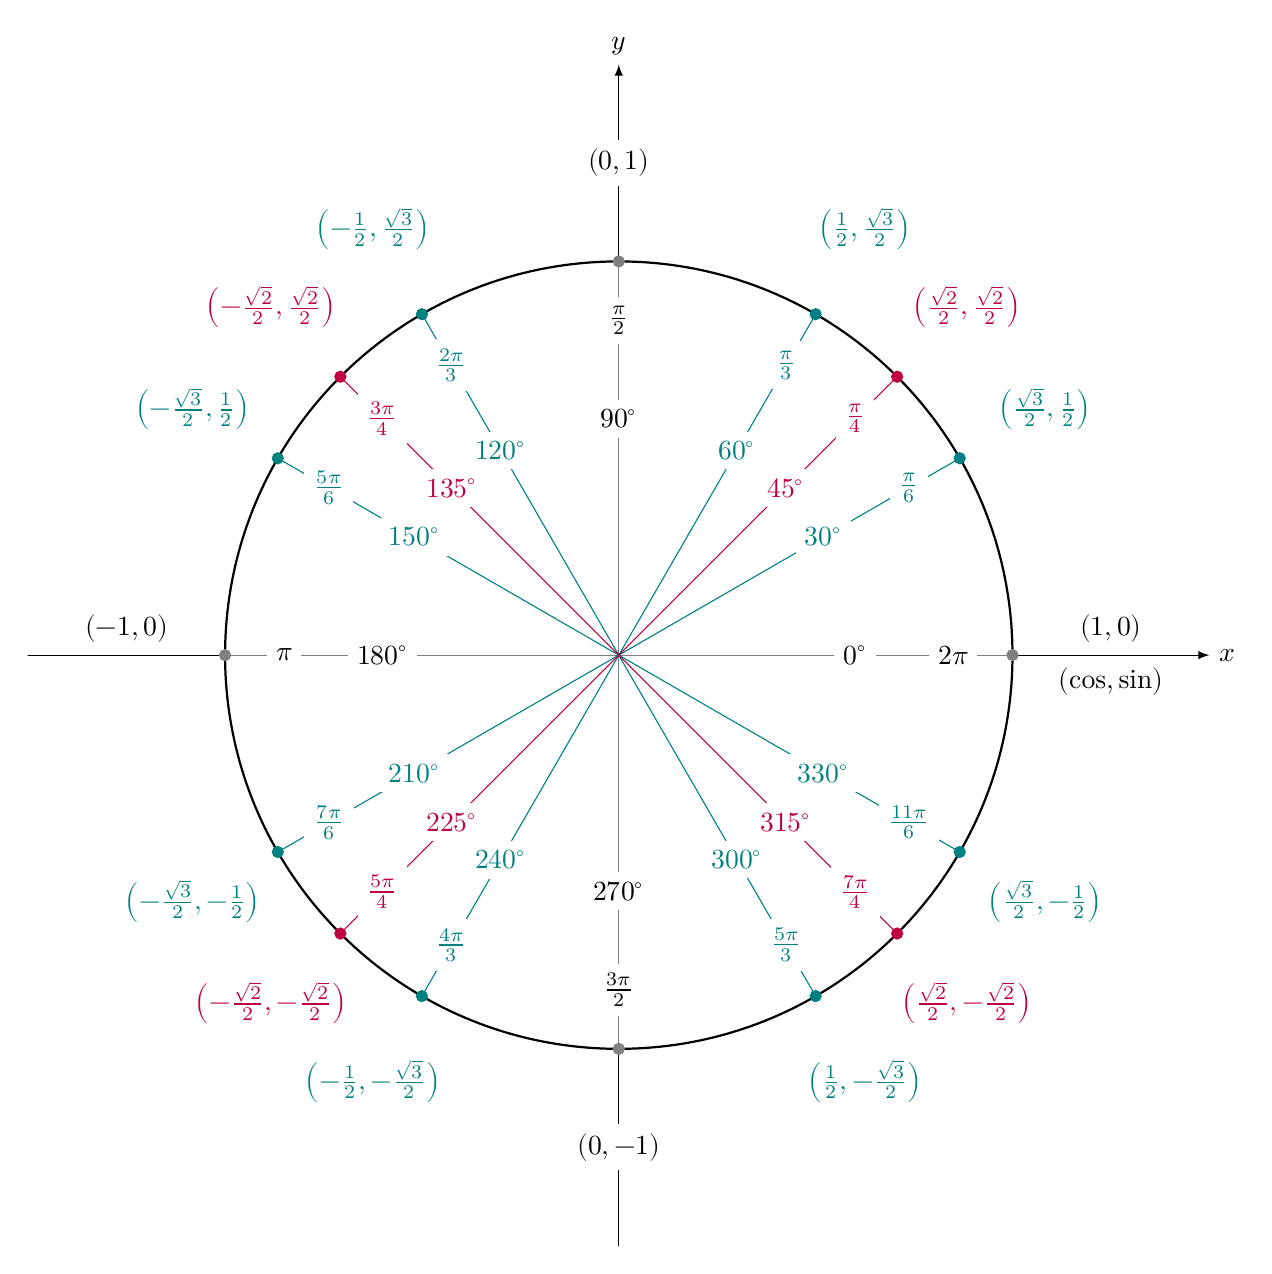
\begin{tikzpicture}[scale=5,cap=round,>=latex]
        % draw the coordinates
        \draw[->] (-1.5cm,0cm) -- (1.5cm,0cm) node[right,fill=white] {$x$};
        \draw[->] (0cm,-1.5cm) -- (0cm,1.5cm) node[above,fill=white] {$y$};

        % draw the unit circle
        \draw[thick] (0cm,0cm) circle(1cm);

        \foreach \x in {0,90, 180, 270} {
                % lines from center to point
                \draw[gray] (0cm,0cm) -- (\x:1cm);
                % dots at each point
                \filldraw[gray] (\x:1cm) circle(0.4pt);
                % draw each angle in degrees
                \draw (\x:0.6cm) node[fill=white] {$\x^\circ$};
        }
         \foreach \x in {30, 60, 120, 150, 210, 240, 300, 330} {
                % lines from center to point
                \draw[teal] (0cm,0cm) -- (\x:1cm);
                % dots at each point
                \filldraw[teal] (\x:1cm) circle(0.4pt);
                % draw each angle in degrees
                \draw[teal] (\x:0.6cm) node[fill=white] {$\x^\circ$};
        }
        
         \foreach \x in {45,135,225,315} {
                % lines from center to point
                \draw[purple] (0cm,0cm) -- (\x:1cm);
                % dots at each point
                \filldraw[purple] (\x:1cm) circle(0.4pt);
                % draw each angle in degrees
                \draw[purple] (\x:0.6cm) node[fill=white] {$\x^\circ$};
        }
       
            
            

        % Beschriftungen Radians
        \foreach \x/\xtext in {
            90/\frac{\pi}{2},
            180/\pi,
            270/\frac{3\pi}{2},
            360/2\pi}
                \draw (\x:0.85cm) node[fill=white] {$\xtext$};
                
            
            \foreach \x/\xtext in {
            30/\frac{\pi}{6},
            60/\frac{\pi}{3},
            120/\frac{2\pi}{3},
            150/\frac{5\pi}{6},
            210/\frac{7\pi}{6},
            240/\frac{4\pi}{3},
            300/\frac{5\pi}{3},
            330/\frac{11\pi}{6}
            }
                \draw[teal] (\x:0.85cm) node[fill=white] {$\xtext$};
            
            \foreach \x/\xtext in {
            45/\frac{\pi}{4},
            135/\frac{3\pi}{4},
            225/\frac{5\pi}{4},
            315/\frac{7\pi}{4}
           }
                \draw[purple] (\x:0.85cm) node[fill=white] {$\xtext$};
                
            
        \foreach \x/\xtext/\y in {
            45/\frac{\sqrt{2}}{2}/\frac{\sqrt{2}}{2},
            135/-\frac{\sqrt{2}}{2}/\frac{\sqrt{2}}{2},
            225/-\frac{\sqrt{2}}{2}/-\frac{\sqrt{2}}{2},
            315/\frac{\sqrt{2}}{2}/-\frac{\sqrt{2}}{2}
        }
            \draw[purple] (\x:1.25cm) node[fill=white] {$\left(\xtext,\y\right)$};
        
        \foreach \x/\xtext/\y in {
            % the coordinates for the first quadrant
            30/\frac{\sqrt{3}}{2}/\frac{1}{2},
            60/\frac{1}{2}/\frac{\sqrt{3}}{2},
            % the coordinates for the second quadrant
            150/-\frac{\sqrt{3}}{2}/\frac{1}{2},
            120/-\frac{1}{2}/\frac{\sqrt{3}}{2},
            % the coordinates for the third quadrant
            210/-\frac{\sqrt{3}}{2}/-\frac{1}{2},
            240/-\frac{1}{2}/-\frac{\sqrt{3}}{2},
            % the coordinates for the fourth quadrant
            330/\frac{\sqrt{3}}{2}/-\frac{1}{2},
            300/\frac{1}{2}/-\frac{\sqrt{3}}{2}}
                \draw[teal] (\x:1.25cm) node[fill=white] {$\left(\xtext,\y\right)$};

        % draw the horizontal and vertical coordinates
        % the placement is better this way
        \draw (-1.25cm,0cm) node[above=1pt] {$(-1,0)$}
              (1.25cm,0cm)  node[above=1pt] {$(1,0)$}
              (1.25cm,0cm)  node[below=1pt] {$(\cos,\sin)$}
              (0cm,-1.25cm) node[fill=white] {$(0,-1)$}
              (0cm,1.25cm)  node[fill=white] {$(0,1)$};
\end{tikzpicture}}
\end{center}

\resizebox{\columnwidth}{!}{\begin{tabular}{|c@{\hspace{3pt}}|c@{\hspace{3pt}}|c|c|c|c|c|c|c|c|}
        \hline
        Degrees &$0^\circ$ &$30^\circ$ &$45^\circ$ &$60^\circ$ &$90^\circ$ &$120^\circ$ &$135^\circ$ &$150^\circ$ &$180^\circ$\\
        \hline
        $\varphi$ &$0$ &$\frac{\pi}{6}$ &$\frac{\pi}{4}$ &$\frac{\pi}{3}$ &$\frac{\pi}{2}$ &$\frac{2\pi}{3}$ &$\frac{3\pi}{4}$ &$\frac{5\pi}{6}$ &$\pi$\\
        \hline
        $\sin(\varphi)$ &$0$ &$\frac{1}{2}$ &$\frac{\sqrt{2}}{2}$ &$\frac{\sqrt{3}}{2}$ &$1$ &$\frac{\sqrt{3}}{2}$ &$\frac{\sqrt{2}}{2}$ &$\frac{1}{2}$ &$0$\\
        \hline
        $\cos(\varphi)$ &$1$ &$\frac{\sqrt{3}}{2}$ &$\frac{\sqrt{2}}{2}$ &$\frac{1}{2}$ &$0$ &$-\frac{1}{2}$ &$-\frac{\sqrt{2}}{2}$ &$-\frac{\sqrt{3}}{2}$ &$-1$\\
        \hline
        $\tan(\varphi)$ &$0$ &$\frac{\sqrt{3}}{3}$ &$1$ &$\sqrt{3}$ &$\pm \infty$ &-$\sqrt{3}$ &$-1$ &$-\frac{\sqrt{3}}{3}$ &$0$\\
        \hline 
    \end{tabular}}
    \begin{itemize}
    \item$\sin(x) = x + o(x)$
    \item $\sin(x+y)\sin(x-y) = \cos^2(y) - \cos^2(x) = \sin^2(x) - \sin^2(y)$
    \item $\cos(x+y)\cos(x-y) = \cos^2(y) - \sin^2(x) = \cos^2(x) - \sin^2(y)$
    \item $\sin{x}\cos{y} = \frac{1}{2}(\sin(x+y) + \sin(x-y))$ 
    \item $\cos{x}\cos{y} = \frac{1}{2}(\cos(x+y) + \cos(x-y))$
    \item  $\sin{x}\sin{y} = \frac{1}{2}(\cos(x-y)-\cos(x+y))$
    \item $\cos(x)^2 + \sin(x)^2 = 1$
    \item $\cos(\pi-x) = -\cos(x)$, $\sin(\pi-x) = \sin(x)$
    \item $\cos(x+\pi) = -\cos(x)$, $\sin(x+\pi) = -\sin(x)$
    \item $\cos(2x) = \cos^2(x) - \sin^2(x) = 1-2\sin^2(x) = 2\cos^2(x) - 1$
    \item $\sin(2x) = 2\sin(x)\cos(x)$ \ $\tan(2x) = \frac{2\tan(x)}{1-\tan^2(x)}$
    \item $\sin(\frac{x}{2}) = \sqrt{\frac{1-\cos(x)}{2}}$ \ $\cos(\frac{x}{2}) = \sqrt{\frac{1+\cos(x)}{2}}$
    \item $\tan(\frac{x}{2}) = \frac{1-\cos(x)}{\sin(x)} = \frac{\sin(x)}{1+\cos(x)}$ \ $\cot(\frac{x}{2}) = \frac{1+\cos(x)}{\sin(x)} = \frac{\sin(x)}{1-\cos(x)}$
    \item $\sin^2(x) = \frac{1-\cos(2x)}{2}$
    \ $\cos^2(x) = \frac{1+\cos(2x)}{2}$
    \item $\tan(\pi + x) = \tan(x)$
    \item $-\sin(-x) = \sin(x), \cos(-x) = \cos(x), \tan(-x) = -\tan(x)$
    \item For all $(a,b)\in \R^2$, such that $a^2+b^2 = 1$, there is $x\in\R$, such that $a = \cos(x)$, $b = \sin(x)$.
    \item $\sin(x) = \frac{2\tan(x/2)}{1+\tan^2(x/2)}$
    \ $\cos(x) = \frac{1-\tan^2(x/2)}{1+\tan^2(x/2)}$
    \item $\sin(x) = \frac{e^{ix} - e^{-ix}}{2i}$
    \ $\cos(x) = \frac{e^{ix} + e^{-ix}}{2}$
    \item $\int_0^{2\pi} \sin(t)\cdot \cos(t) dt = \int_0^{2\pi} \sin(t) dt = \int_0^{2\pi} \cos(t) dt = 0$
    \item $\int \sin^2(x) dx = \frac{1}{2} (x-\sin(x) \, \cos(x))$
    \item $\int \cos^2(x) dx = \frac{1}{2} (x+\sin(x) \, \cos(x))$
    \item $\int x \sin(x) dx = \sin (x)-x \cos (x)$
    \item $\int x \cos(x) dx = x \sin (x)+\cos (x)$
    \item $\sin(\arccos(x)) = \sqrt{1-x^{2}}$ \ $\sin(\arctan(x)) = \frac{x}{\sqrt{1+x^{2}}}$ 
    \item $\cos(\arctan(x)) = \frac{1}{\sqrt{1+x^{2}}}$ \ $\cos(\arcsin(x)) = \sqrt{1-x^{2}}$ 
    \item $\tan(\arcsin(x)) = \frac{x}{\sqrt{1-x^{2}}}$ \ $\tan(\arccos(x)) = \frac{\sqrt{1-x^{2}}}{x}$
    \item $\cosh(x) := \frac{e^x + e^{-x}}{2}$ \ $\sinh x := \frac{e^x - e^{-x}}{2}$ \ $\tanh x := \frac{e^x - e^{-x}}{e^x + e^{-x}}$
    \item $\sinh(z) = -\sinh(-z)$ \ $\cosh(z) = \cosh(-z)$ 
    \item $\sinh(z) = \sinh(z + 2\pi i)$ \ $\cosh(z) = \cosh(z+ 2\pi i)$
    \item $\sinh(z_1 \pm z_2) = \sinh(z_1) \cdot \cosh(z_2) \pm \sinh(z_2) \cdot \cosh(z_1)$
    \item $\sinh(z_1 \pm z_2) = \cosh(z_1) \cdot \cosh(z_2) \pm \sinh(z_2) \cdot \sinh(z_1)$
    \item $\tanh(z_1 \pm z_2) = \frac{\tanh(z_1) \pm \tanh(z_2)}{1 \pm \tanh(z_1)\cdot \tanh(z_2)}$
    \end{itemize}

\textbf{Prove if $f$ is differentiable at $x_0$}

$f$ continuous at $x_0$? No $\Rightarrow$ Not differentiable.\\
$\Downarrow$ Yes\\
Is $f$ partially differentiable at $x_0$, does $\partial_{x_i}f(x_0)$ exist for all $i$?
No $\Rightarrow$ Not differentiable.\\
$\Downarrow$ Yes\\
Are all partial derivatives continuous at $x_0$? Yes $\Rightarrow f$ is differentiable at $x_0$ with $df(x_0)=J_f(x_0).$\\
$\Downarrow$ No\\
Does a linear mapping $u$ exist, such that 
$\displaystyle\lim_{x\rightarrow x_0 \atop x\neq 0} \frac{f(x)-f(x_0)-u(x-x_0)}{||x-x_0||}=0$?\\
Yes $\Rightarrow$ $f$ is differentiable at $x_0$.\\
No $\Rightarrow f$ is not differentiable at $x_0$ *cries*.

\textbf{Primitives and Derivatives}

$\mathlarger{\int (ax+b)^s\;dx= \frac{1}{a(s+1)}(ax+b)^{s+1} + C,\;s\neq -1}$\\
$\mathlarger{\int \frac{1}{ax+b}dx=\frac{1}{a}\;log|ax+b|+C}$\\
$\mathlarger{\int (ax^p+b)^sx^{p-1}\;dx = \frac{(ax^p+b)^{s+1}}{ap(s+1)}+C,\;s\neq -1, a \neq 0}$\\
$\mathlarger{\int (ax^p+b)^{-1}x^{p-1}\;dx=\frac{1}{ap}log|ax^p+b|+C,\;a\neq 0,p\neq 0}$\\
$\mathlarger{\int \frac{ax+b}{cx+d}dx=\frac{ax}{c}- \frac{ad-bc}{c^2} log|cx+d|+C}$\\
$\mathlarger{\int \frac{1}{x^2+a^2}dx=\frac{1}{a}arctan(\frac{x}{a})+C}$\\
$\mathlarger{\int \frac{1}{x^2-a^2}dx=\frac{1}{2a}log\Bigl|\frac{x-a}{x+a}\Bigl|}$\\
$\mathlarger{\int \sqrt{a^2+x^2}\;dx=\frac{x}{2}\sqrt{a^2+x^2}+\frac{a^2}{2} log(x+\sqrt{a^2+x^2})+C}$\\
$\mathlarger{\int \sqrt{a^2-x^2}\;dx= \frac{x}{2}\sqrt{a^2-x^2}+\frac{a^2}{2}arcsin\Bigl(\frac{x}{|a|}\Bigl)+C}$\\
$\mathlarger{\int \sqrt{x^2-a^2}\;dx= \frac{x}{2}\sqrt{x^2-a^2}-\frac{a^2}{2}log|x+\sqrt{x^2-a^2}|+C}$\\
$\mathlarger{\int \frac{1}{\sqrt{x^2-a^2}}\;dx=log(x+\sqrt{a^2+x^2})+C}$\\
$\mathlarger{\int \frac{1}{\sqrt{x^2-a^2}}\;dx=log|x+\sqrt{x^2-a^2}|+C}$\\
$\mathlarger{\int \frac{1}{\sqrt{a^2-x^2}}\;dx=arcsin\Bigl(\frac{x}{|a|}\Bigl)+C}$\\
$\mathlarger{\int e^{kx}\;dx=\frac{1}{k}e^{kx}+C}$\\
$\mathlarger{\int a^{kx}\;dx=\frac{1}{k*log(a)}a^{kx}+C}$\\
$\mathlarger{\int e^{ax}p(x)\;dx=e^{ax}(a^{-1}p(x)-a^{-2}p'(x)+a^{-3}p''(x)-\dots}$\\
$\mathlarger{+(-1)^na^{-n-1}p^{(n)}(x))+C}$, $a\neq 0$, $p$: Polynome of degree $n$\\
$\mathlarger{\int e^{kx}sin(ax+b)\;dx=\frac{e^{kx}}{a^2+k^2}\Bigl(k\;sin(ax+b)- a\;cos(ax+b)\Bigl)+C}$\\
$\mathlarger{\int e^{kx}cos(ax+b)\;dx=\frac{e^{kx}}{a^2 + k^2}\Bigl(k\;cos(ax+b)...}$\\
$\mathlarger{...+a\;sin(ax+b)\Bigl)+C}$\\
$\mathlarger{\int log|x|\;dx= x(log|x|-1)+C}$\\
$\mathlarger{\int x^k log(x)\;dx=\frac{x^{k+1}}{k+1}\Bigl(log(x)-\frac{1}{k+1}\Bigl)+C}$, $k\neq -1$\\
$\mathlarger{\int x^{-1}log(x)\;dx= \frac{1}{2}(log(x))^2 + C}$\\
$\mathlarger{\int sin(ax+b)\;dx=-\frac{1}{a}cos(ax+b)+C}$\\
$\mathlarger{\int cos(ax+b)\;dx=\frac{1}{a}sin(ax+b)+C}$\\
$\mathlarger{\int sin^2(x)\;dx= \frac{1}{2}(x-sin(x)cos(x))+C}$\\
$\mathlarger{\int cos^2(x)\;dx= \frac{1}{2}(x+sin(x)cos(x))+C}$\\
$\mathlarger{\int tan^2(x)\;dx= tan(x)-x+C}$\\
$\mathlarger{\int \frac{1}{sin(x)}\;dx=log\Bigl|tan\frac{x}{2}\Bigl|+C}$\\
$\mathlarger{\int \frac{1}{cos(x)}\;dx=log\Bigl|tan\Bigl(\frac{x}{2}+\frac{\pi}{4}\Bigl)\Bigl|+C}$\\
$\mathlarger{\int \frac{1}{tan(x)}\;dx=log|sin(x)|+C}$\\

$\mathlarger{\int_0^{2\pi} sin(mx)cos(nx)\;dx=0}$, $m,n\in \mathbb{Z}$\\
$\mathlarger{\int_0^\infty \frac{sin(ax)}{x}\;dx=\frac{\pi}{2},\;a>0}$\\
$\mathlarger{\int_0^\infty sin(x^2)\;dx=\int_0^\infty cos(x^2)\;dx=\frac{1}{2}\sqrt{\frac{\pi}{2}}}$\\
$\mathlarger{\int_0^\infty e^{-ax}x^n\;dx= \frac{n!}{a^{n+1}},\;a>0}$\\
$\mathlarger{\int_0^\infty e^{-ax^2}\;dx=\frac{1}{2}\sqrt{\frac{\pi}{a}},\;a>0}$\\

$\textbf{Differentiable }\implies\textbf{ Continuous }\implies \textbf{ Integrable}$

\resizebox{\columnwidth}{!}{\begin{tabular}{c|c|c}
  $\mathbf{f'(x)}$ & $\mathbf{f(x)}$ & $\mathbf{F(x)}$ \\[0.5em] \hline
  0 & c ($c\in\R)$ & $cx$ \\[0.5em]
  $c$ & $cx$ &$\frac{c}{2}x^2$ \\[0.5em]
  $r\cdot x^{r-1}$ & $x^r (r\in \R \backslash \{-1\}$ & $\frac{x^{r+1}}{r+1}$ \\[0.5em]
  $\frac{-1}{x^2} = -x^{-2}$ & $\frac{1}{x}=x^{-1}$ & $\log |x| $ \\[0.5em]
  $\frac{1}{2 \sqrt{x}} = -x^{-2}$ & $\sqrt{x} = x^{\frac{1}{2}}$ & $\frac{2}{3}x^{\frac{3}{2}}$ \\[0.5em]
  $\cos x$ & $\sin x$  & $-\cos x$ \\[0.5em]
  $-\sin x$ & $\cos x$ & $\sin x$\\[0.5em]
  $1+\tan^2x = \frac{1}{\cos^2x}$ & $\tan x$ & $-\log|\cos x|$\\[0.5em]
  $-\frac{1}{\sin^2(x)}$ & $\cot x$ & $\log|\sin x|$\\[0.5em]
  $e^x$ & $e^x$ & $e^x$\\[0.5em]
  $c\cdot e^{cx}$ & $e^{cx}$ & $\frac{1}{c}e^{cx}$\\[0.5em]
  $\log a \cdot a^x$ & $a^x$ & $\frac{a^x}{\log a}$\\[0.5em]
  $\frac{1}{x}$ & $\log|x|$ & $x(\log|x|-1)$ \\[0.5em]
  $\frac{1}{\log a\cdot x}$ & $\log_a |x|$ & $\frac{x}{\log a}(\log|x|-1)$\\[0.5em]
   & & = $x(\log_a|x|-\log_ae)$\\[0.5em]
  $\frac{1}{\sqrt{1-x^2}}$ & $\arcsin x$ & $x\arcsin x + \sqrt{1-x^2}$\\[0.5em]
  $-\frac{1}{\sqrt{1-x^2}}$ & $\arccos x$ &  $x\arccos x - \sqrt{1-x^2}$\\[0.5em]
  $\frac{1}{1+x^2}$ & $\arctan x$ & $x\arctan x - \frac{1}{2}\log(1+x^2)$\\[0.5em]
  $\sinh(x)$ & $\cosh(x)$ & - \\[0.5em]
  $\cosh(x)$ & $\sinh(x)$ & -\\[0.5em]
  $\frac{1}{\cosh^2(x)}$ & $\tanh(x)$ & $\log(\cosh(x))$\\[1em]
  $2 \sin(x)\cos(x)$ & $\sin^2(x)$ & $\frac{1}{2}(x-\sin(x)\cos(x))$ \\[.5em]
  $-2\sin(x)\cos(x)$ & $\cos^2(x)$ & $\frac{1}{2}(x+\sin(x)\cos(x))$ \\[.5em]
  $\frac{2 \sin(x)}{\cos^3(x)}$ & $\tan^2(x)$ & $\tan(x) - x$\\[.5em]
  $\frac{1}{\sqrt {x^2+1}}$& $\operatorname{arsinh} x$ & $x \operatorname{arsinh} x -\sqrt{x^2+1}$\\
  $\frac{1}{\sqrt {x^2-1}} \quad (x>1)$&$\operatorname{arcosh} x$ & $x \operatorname{arcosh} x -\sqrt{x^2-1}$\\
  $\frac{1}{1-x^2} \quad (\left| x \right|<1)$&$\operatorname{artanh} x$ & $x \operatorname{artanh} x +\frac{1}{2}\ln{\left(1-x^2\right)}$\\
  $\frac{1}{1-x^2} \quad (\left| x \right|>1)$&$\operatorname{arcoth} x$ & $x \operatorname{arcoth} x +\frac{1}{2}\ln{\left(x^2-1\right)}$\\ 
\end{tabular}}

\end{multicols*}
\end{document}
